% PlanWise -- User Guide (English).
% Build:  latexmk -xelatex user-guide.tex   (or: xelatex user-guide.tex, twice)
% Figures come from capture_screenshots.py (English demo instance, see research/demo_video).
\documentclass[11pt,a4paper,oneside]{report}

% ---------------------------------------------------------------- fonts & layout
\usepackage{fontspec}
\setmainfont{Segoe UI}[BoldFont={Segoe UI Semibold}, ItalicFont={Segoe UI Italic}, BoldItalicFont={Segoe UI Semibold Italic}]
\setsansfont{Segoe UI}[BoldFont={Segoe UI Semibold}]
\setmonofont{Consolas}[Scale=0.92]
\usepackage[a4paper, left=2.3cm, right=2.3cm, top=2.4cm, bottom=2.4cm, headheight=14pt]{geometry}
\usepackage{microtype}
\usepackage{parskip}
\setlength{\parskip}{0.55em}
\linespread{1.12}
\setlength{\emergencystretch}{2.5em}   % let lines with long words stretch instead of overflowing

\usepackage[table]{xcolor}
\definecolor{brand}{HTML}{1E56A0}
\definecolor{brandsoft}{HTML}{EAF1FB}
\definecolor{ink}{HTML}{1F2937}
\definecolor{muted}{HTML}{6B7280}
\definecolor{callout}{HTML}{E11D48}
\definecolor{tipbg}{HTML}{ECFDF5}\definecolor{tipfg}{HTML}{047857}
\definecolor{notebg}{HTML}{EFF6FF}\definecolor{notefg}{HTML}{1D4ED8}
\definecolor{warnbg}{HTML}{FFF7ED}\definecolor{warnfg}{HTML}{C2410C}
\definecolor{rule}{HTML}{D1D5DB}
\color{ink}

\usepackage{graphicx}
\graphicspath{{figures/}}
\usepackage{float}
\usepackage[font=small, labelfont={bf,color=brand}, skip=6pt]{caption}
\usepackage{booktabs, tabularx, longtable, array, multirow, makecell}
\usepackage{enumitem}
\setlist{itemsep=0.25em, topsep=0.3em, leftmargin=1.4em}
\usepackage{tikz}
\usetikzlibrary{positioning, arrows.meta, shapes.geometric, calc}
\usepackage[most]{tcolorbox}
\usepackage{fontawesome5}
\usepackage{needspace}
\usepackage{etoolbox}

% ---------------------------------------------------------------- headings
\usepackage{titlesec}
\titleformat{\chapter}[display]
  {\normalfont\color{brand}}
  {\large\sffamily\bfseries\MakeUppercase{\chaptertitlename}\ \thechapter}
  {4pt}
  {\Huge\bfseries}[\vspace{2pt}{\color{brand}\titlerule[1.2pt]}]
\titlespacing*{\chapter}{0pt}{-10pt}{22pt}
\titleformat{\section}{\Large\bfseries\color{brand}}{\thesection}{0.8em}{}
\titleformat{\subsection}{\large\bfseries\color{ink}}{\thesubsection}{0.7em}{}
\titleformat{\subsubsection}{\normalsize\bfseries\color{ink}}{}{0em}{}
\titlespacing*{\section}{0pt}{18pt}{6pt}
\titlespacing*{\subsection}{0pt}{14pt}{4pt}
\setcounter{secnumdepth}{2}
\setcounter{tocdepth}{1}

\usepackage{fancyhdr}
\pagestyle{fancy}
\fancyhf{}
\fancyhead[L]{\small\color{muted}PlanWise User Guide}
\fancyhead[R]{\small\color{muted}\leftmark}
\fancyfoot[C]{\small\color{muted}\thepage}
\renewcommand{\headrulewidth}{0.4pt}
\renewcommand{\headrule}{{\color{rule}\hrule height\headrulewidth}}
\renewcommand{\chaptermark}[1]{\markboth{#1}{}}
\fancypagestyle{plain}{\fancyhf{}\fancyfoot[C]{\small\color{muted}\thepage}\renewcommand{\headrulewidth}{0pt}}

\usepackage{tocloft}
\renewcommand{\cftchapfont}{\bfseries\color{brand}}
\renewcommand{\cftchappagefont}{\bfseries\color{brand}}
\setlength{\cftbeforechapskip}{6pt}

\usepackage[hidelinks, bookmarksnumbered, pdfusetitle]{hyperref}
\hypersetup{pdftitle={PlanWise User Guide}, pdfauthor={PlanWise}, pdfsubject={Production scheduling for an alloy wheel plant}}
\usepackage{bookmark}

% ---------------------------------------------------------------- guide macros
\newcommand{\ui}[1]{\textbf{\textsf{#1}}}                       % a label as written on screen
\newcommand{\menu}[1]{\textbf{\textsf{#1}}}
\newcommand{\code}[1]{\texttt{#1}}
\newcommand{\kbd}[1]{\tikz[baseline=(k.base)]\node[draw=rule, fill=gray!6, rounded corners=2pt, inner xsep=3.5pt, inner ysep=1.6pt, font=\footnotesize\ttfamily](k){#1};}
\newcommand{\callout}[1]{\tikz[baseline=(c.base)]\node[circle, fill=callout, text=white, font=\scriptsize\bfseries, inner sep=0pt, minimum size=1.35em, draw=white, line width=0.6pt](c){#1};}
\newcommand{\term}[1]{\emph{#1}}

\newtcolorbox{tip}{enhanced, breakable, colback=tipbg, colframe=tipbg, coltext=ink, boxrule=0pt, leftrule=3pt,
  colbacktitle=tipbg, sharp corners, left=8pt, right=8pt, top=5pt, bottom=5pt, borderline west={3pt}{0pt}{tipfg},
  before upper={\textcolor{tipfg}{\faLightbulb[regular]\ \textbf{Tip.}}\ }}
\newtcolorbox{note}{enhanced, breakable, colback=notebg, colframe=notebg, coltext=ink, boxrule=0pt, sharp corners,
  left=8pt, right=8pt, top=5pt, bottom=5pt, borderline west={3pt}{0pt}{notefg},
  before upper={\textcolor{notefg}{\faInfoCircle\ \textbf{Note.}}\ }}
\newtcolorbox{warning}{enhanced, breakable, colback=warnbg, colframe=warnbg, coltext=ink, boxrule=0pt, sharp corners,
  left=8pt, right=8pt, top=5pt, bottom=5pt, borderline west={3pt}{0pt}{warnfg},
  before upper={\textcolor{warnfg}{\faExclamationTriangle\ \textbf{Caution.}}\ }}
\newtcolorbox{steps}[1][]{enhanced, breakable, colback=white, colframe=rule, boxrule=0.5pt, arc=2pt,
  left=8pt, right=8pt, top=6pt, bottom=6pt, title={\faListOl\ \ #1}, fonttitle=\bfseries\color{brand}, colbacktitle=brandsoft, coltitle=brand}

% \shot[width]{file}{caption}{label}
\newcommand{\shot}[4][\linewidth]{%
  \begin{figure}[H]\centering
  \includegraphics[width=#1]{#2}
  \caption{#3}\label{fig:#4}
  \end{figure}}
% framed screenshot (dialogs, crops)
\newcommand{\shotf}[4][0.7\linewidth]{%
  \begin{figure}[H]\centering
  {\setlength{\fboxsep}{0pt}\setlength{\fboxrule}{0.4pt}\color{rule}\fbox{\includegraphics[width=#1]{#2}}}
  \caption{#3}\label{fig:#4}
  \end{figure}}

% callout legend: \begin{callouts} \item[1] text ... \end{callouts}
\newenvironment{callouts}{\begin{description}[leftmargin=2.2em, labelwidth=1.6em, labelsep=0.5em, font=\normalfont, itemsep=0.2em]\renewcommand{\makelabel}[1]{\callout{##1}}}{\end{description}}

\rowcolors{2}{gray!5}{white}
\renewcommand{\arraystretch}{1.25}

% ================================================================= document
\begin{document}

\begin{titlepage}
\begin{tikzpicture}[remember picture, overlay]
  \fill[brand] (current page.north west) rectangle ([yshift=-9.2cm]current page.north east);
  \fill[brand!80!black] ([yshift=-9.2cm]current page.north west) rectangle ([yshift=-9.5cm]current page.north east);
  \node[anchor=north west, text=white, font=\sffamily\bfseries\fontsize{14}{16}\selectfont] at ([xshift=2.3cm, yshift=-2.2cm]current page.north west) {\faCalendarCheck[regular]\ \ PlanWise};
  \node[anchor=north west, text=white, font=\sffamily\bfseries\fontsize{40}{44}\selectfont, align=left] at ([xshift=2.3cm, yshift=-3.6cm]current page.north west) {User Guide};
  \node[anchor=north west, text=white!88!brand, font=\sffamily\fontsize{15}{19}\selectfont, align=left, text width=15cm] at ([xshift=2.3cm, yshift=-5.6cm]current page.north west)
    {Reasonable production scheduling for a five-stage alloy wheel plant: from the order book to a committed, explainable schedule};
\end{tikzpicture}
\vspace*{9.6cm}

{\large\color{muted} For production planners, shift supervisors and plant engineers}

\vspace{1.2cm}
\begin{tabularx}{\linewidth}{@{}lX@{}}
\rowcolor{white}\textbf{Software} & PlanWise web application (English interface) \\
\rowcolor{white}\textbf{Edition} & November 2026 \\
\rowcolor{white}\textbf{Example plant} & Riverside Alloy Wheels -- Plant 1 (demonstration data) \\
\rowcolor{white}\textbf{Context} & CO5103 Management Information Systems -- Reasonable Scheduling Agent \\
\end{tabularx}

\vfill
{\small\color{muted} The screenshots in this guide were taken from a demonstration instance with realistic but fictional data. Company and customer names are invented. Figures such as on-time counts and costs vary from one solver run to the next.}
\end{titlepage}

\pagenumbering{roman}
\tableofcontents
\clearpage
\pagenumbering{arabic}

\chapter{Introduction}\label{ch:intro}

\section{What PlanWise does}

PlanWise is a scheduling agent for a make-to-order plant. It takes the orders customers have placed, the
plant's machines, shifts and rules, and the stock that is already on the floor, and it builds a
\term{reasonable} production schedule for the next planning period: one that is feasible on every machine,
delivers as many orders on time as possible, keeps finished goods above their safety level, and does not open
more shifts or changeovers than necessary.

The planner stays in charge. PlanWise proposes several schedules (\term{options}), explains how each was
built and why an order is late, lets the planner edit any of them by hand, and records which one was
committed and why. The committed schedule then becomes printable work orders for the shop floor, and can be
replanned in minutes when a machine breaks down.

The example used throughout this guide is an alloy wheel plant with five stages:

\begin{center}
\begin{tikzpicture}[stage/.style={draw=brand, fill=brandsoft, rounded corners=3pt, minimum width=2.45cm, minimum height=1.1cm, align=center, font=\small\bfseries}, arr/.style={-{Stealth[length=2.4mm]}, thick, brand}]
\node[stage] (c) {Casting\\[-1pt]{\scriptsize\normalfont 2 die-casting cells}};
\node[stage, right=0.55cm of c] (h) {Heat treatment\\[-1pt]{\scriptsize\normalfont 2 T6 furnaces, 24/7}};
\node[stage, right=0.55cm of h] (m) {Machining\\[-1pt]{\scriptsize\normalfont 2--3 CNC lathes}};
\node[stage, right=0.55cm of m] (p) {Painting\\[-1pt]{\scriptsize\normalfont conveyor line}};
\node[stage, right=0.55cm of p] (q) {Test \& packing\\[-1pt]{\scriptsize\normalfont 1 station}};
\draw[arr] (c) -- (h); \draw[arr] (h) -- (m); \draw[arr] (m) -- (p); \draw[arr] (p) -- (q);
\end{tikzpicture}
\end{center}

Four products (17-inch front and rear wheels, each in silver and matte black) pass through all five stages.
Each stage works in fixed-size \term{runs} (for example 16 wheels per casting run, 24 per furnace load). Front
and rear wheels share their semi-finished stock up to machining; the colour is only decided at the paint line.
Heat treatment takes eight hours per load and is the plant's bottleneck.

\section{Who this guide is for}

\begin{itemize}
  \item \textbf{Production planners} prepare each period, generate and compare schedules, edit and commit
        one, and replan after incidents. Chapters~\ref{ch:today}--\ref{ch:variants} are written for them.
  \item \textbf{Plant or industrial engineers} maintain the factory set-up: stages, products, machines, molds,
        shifts and the policies that define a good schedule (Chapter~\ref{ch:factory}).
  \item \textbf{Shift supervisors} mainly use the work orders of the committed schedule
        (Section~\ref{sec:work-orders}).
  \item \textbf{Analysts and researchers} use the analysis views and the Advanced section to compare
        algorithms on the same data (Chapters~\ref{ch:analysis} and~\ref{ch:advanced}).
\end{itemize}

\section{Conventions used in this guide}

\begin{itemize}
  \item Labels exactly as they appear on screen are set in bold sans-serif, for example \ui{Generate options}
        or \ui{Save \& check}.
  \item Keys are shown as \kbd{Ctrl}\,\kbd{K}.
  \item Codes and identifiers are set in monospace, for example \code{F\_SILVER} or \code{CNC\_1}.
  \item Numbered red markers such as \callout{1} \callout{2} \callout{3} on a screenshot are explained in the
        list directly below that figure.
  \item Boxes mark tips \faLightbulb[regular], notes \faInfoCircle{} and cautions \faExclamationTriangle.
\end{itemize}

\section{Key concepts}\label{sec:concepts}

PlanWise separates data by \emph{how often it changes}. Getting this idea right makes every screen easier to
understand.

\begin{center}
\begin{tabularx}{\linewidth}{>{\bfseries}p{3.1cm}Xp{3.2cm}}
\toprule
\rowcolor{white}Layer & What it contains & Changes \\
\midrule
Factory set-up & Stages, run sizes, products and routes, machines with rates and changeovers, molds, shifts, rest days, holidays, weekly maintenance, objective policies. Every save creates an immutable \term{version}. & A few times a year (Factory page) \\
Order book & Every customer order with product, quantity, due date, priority and customer. & Continuously (Order book page) \\
Period inputs & For one planning period: the orders taken from the book, opening stock, mold counters, calendar exceptions, policy and pull-ahead choice. & Every period, usually two weeks (Prepare step) \\
Derived data & Lots, runs per stage, allocation of stock to orders, checkpoints, machine availability. & Never typed in: computed when the period is saved \\
\bottomrule
\end{tabularx}
\end{center}

\subsection*{Glossary of the most important terms}

\begin{description}[style=nextline, leftmargin=1.2em, font=\bfseries\color{brand}]
  \item[Planning period] A window (by default 14 days) that is scheduled as one problem. It takes the factory
        set-up version valid on its start date and the open orders due up to its end.
  \item[Option / schedule] One complete, feasible schedule of a period produced by an algorithm or by a
        planner's edit. A period usually has several options to compare.
  \item[Run (solver run)] One execution of one algorithm on one copy of the data. Each option is the result of
        a run; every run keeps its own data snapshot so it can be reproduced.
  \item[Run (production run)] The unit of work at a stage: a fixed quantity of one item processed on one
        machine, for example ``F\_CAST run 07, 16 units on CAST\_1''.
  \item[Semi-finished code] The identity of goods between stages (for example \code{F\_HEAT}: front wheel,
        heat-treated). Products that share a code share that stock.
  \item[Safety stock] The minimum finished-goods level a product should keep. Falling below it at an
        end-of-day checkpoint counts as \term{safety-stock shortfall}.
  \item[Stock cap] The maximum finished-goods stock the warehouse can hold for a product.
  \item[Policy] The rule that says which schedule is better: a weighted score over objective terms (lateness,
        shortfall, setup time and so on), optionally with ``strictly first'' terms compared before the others.
  \item[Commit] The planner's decision that one option is the plan. It is logged with a mandatory reason.
  \item[Variant] A what-if copy of a period's inputs, used to test a change without touching the main plan.
  \item[Reschedule] A version of a period created after an incident: everything before the \term{cut-off}
        is frozen, the rest is planned again.
  \item[Pull-ahead (build-ahead)] Using spare capacity to make part of the orders due after the period early.
  \item[Look-ahead window] The days after the period whose orders are shown as ``after the period'' and may
        be pulled ahead (28 days by default).
\end{description}

\section{The planning cycle}\label{sec:cycle}

A planning period goes through the same steps every time. The period page shows them as tabs, and the
status badge tells you which step comes next.

\begin{center}
\begin{tikzpicture}[node distance=0.42cm, box/.style={draw=brand, fill=brandsoft, rounded corners=3pt, minimum height=1.05cm, text width=2.35cm, align=center, font=\small}, arr/.style={-{Stealth[length=2.2mm]}, thick, brand}]
\node[box, fill=white] (book) {\textbf{Order book}\\{\scriptsize orders entered once}};
\node[box, right=of book] (create) {\textbf{Create period}\\{\scriptsize dates only}};
\node[box, right=of create] (prep) {\textbf{1 Prepare}\\{\scriptsize orders, stock, calendar}};
\node[box, right=of prep] (gen) {\textbf{2 Options}\\{\scriptsize generate \& rank}};
\node[box, below=0.9cm of gen] (cmp) {\textbf{3 Schedule \& compare}\\{\scriptsize Gantt, why late, edit}};
\node[box, left=of cmp] (commit) {\textbf{4 Commit}\\{\scriptsize with a reason}};
\node[box, left=of commit] (exec) {\textbf{5 Execute}\\{\scriptsize work orders, incidents}};
\node[box, left=of exec, fill=white] (close) {\textbf{Close \& roll over}\\{\scriptsize next period}};
\draw[arr] (book) -- (create); \draw[arr] (create) -- (prep); \draw[arr] (prep) -- (gen); \draw[arr] (gen) -- (cmp);
\draw[arr] (cmp) -- (commit); \draw[arr] (commit) -- (exec); \draw[arr] (exec) -- (close);
\draw[arr, dashed] (close.north) -- (create.south) node[midway, left, font=\scriptsize, text=muted]{closing stock = opening stock};
\draw[arr, dashed] (exec.north) to[bend left=20] node[midway, right, font=\scriptsize, text=muted, align=left]{incident:\\reschedule} (prep.south);
\end{tikzpicture}
\end{center}

\begin{enumerate}
  \item \textbf{Order book.} Sales or the planner enter orders once, by hand or by importing a spreadsheet
        (Chapter~\ref{ch:orders}).
  \item \textbf{Create the period.} Pick a start date. The set-up, shifts, rest days, open orders and the
        projected opening stock come in automatically (Section~\ref{sec:new-period}).
  \item \textbf{Prepare.} Review the orders, correct the opening stock to the physical count, add one-off
        machine stops, pick the policy, and save so the inputs are checked (Chapter~\ref{ch:prepare}).
  \item \textbf{Generate options.} Choose how long to wait; PlanWise runs suitable algorithms in the
        background and recommends the schedules worth considering (Chapters~\ref{ch:generate}
        and~\ref{ch:options}).
  \item \textbf{Schedule \& compare.} Inspect the Gantt chart, compare two options, see why an order is late,
        and edit a schedule by hand if needed (Chapters~\ref{ch:schedule} and~\ref{ch:editing}).
  \item \textbf{Commit.} Choose one option and record why (Section~\ref{sec:commit}).
  \item \textbf{Execute.} Print work orders, replan after incidents, and finally close the period. Its
        projected closing stock becomes the opening stock of the next period (Sections~\ref{sec:work-orders}
        to~\ref{sec:close}).
\end{enumerate}

\chapter{Getting started}\label{ch:start}

\section{Opening PlanWise}

PlanWise is a web application. It consists of a backend (the scheduling service and its database) and the
web interface. Ask your administrator for the address. On a local installation it is:

\centerline{\code{http://localhost:3000}}

Any current browser works (Chrome, Edge, Firefox); a screen at least 1280 pixels wide is recommended,
because the Gantt chart uses the full width.

\begin{note}
For a local installation, an engineer starts both parts with one command from the project folder:
\code{powershell -ExecutionPolicy Bypass -File scripts/dev.ps1}. With Docker, \code{docker compose up
--build} does the same. The API documentation is then available at
\code{http://localhost:8000/api/v1/docs}.
\end{note}

\subsection{Access and roles}

In a development installation no sign-in is needed. In production the backend is protected by keys:

\begin{itemize}
  \item an \textbf{operator} key allows every action (editing data, generating and committing schedules);
  \item a \textbf{reader} key allows viewing only. A reader sees every page, but actions that change data are
        refused, and the schedule editor reports ``This account is read-only and cannot edit schedules.''
\end{itemize}

Every change is recorded with the actor that made it, so committed decisions, set-up versions and imports
can always be traced back.

\section{The screen layout}\label{sec:layout}

Every page shares the same frame (Figure~\ref{fig:today} in the next chapter shows it with callouts).

\begin{description}[style=nextline, leftmargin=1.2em, font=\bfseries\color{brand}]
  \item[Sidebar (left)] The main navigation, grouped as \ui{Schedule} (Today, Planning periods, Order
        book), \ui{Plant set-up} (Factory) and \ui{Advanced} (JSON scenarios, Runs, Aggregate planning).
        The Advanced group is folded by default because planners rarely need it; click its title to open it.
        Your choice is remembered in this browser.
  \item[New button] A shortcut menu for the most common creations (Figure~\ref{fig:new_menu}).
  \item[Factory name] Opens the Factory page. When several plants exist it lets you switch plant.
  \item[Quick search] Opens the command palette (\kbd{Ctrl}\,\kbd{K}) to jump to any page, planning
        period, scenario, recent run or action (Section~\ref{sec:palette}).
  \item[Status box (bottom left)] \ui{System online} when the backend answers, the number of solver runs in
        progress (or \ui{Queue is empty}), the database response time and the time of the latest schedule.
        It turns to \ui{API unreachable} when the backend cannot be reached.
  \item[Top bar] The breadcrumb of the current page, the environment badge (for example
        \ui{development}), the language switch (\ui{EN}/\ui{VI}) and the light/dark theme menu.
\end{description}

\shotf[0.36\linewidth]{new_menu}{The \ui{New} menu: create a planning period, import orders, add one order, or (Advanced) import a JSON scenario, start a single run or create an aggregate plan.}{new_menu}

\section{Language and theme}

The whole interface is bilingual. Click the language button (\ui{EN} or \ui{VI}) in the top bar and pick
\ui{English} or \ui{Tiếng Việt}. The choice is stored in a browser cookie, so it survives reloads, and it
also changes date formats and number formatting. Codes entered by users (order numbers, customer names,
machine names) are shown as they were entered.

The theme menu next to it offers \ui{Light}, \ui{Dark} and \ui{System} (follow the operating system). See
Section~\ref{sec:theme} for a dark-theme screenshot.

\section{The first time: setting up a plant}\label{sec:first-setup}

When no factory exists yet, Today, Order book and Planning periods all show a short message with a
\ui{Set up the factory} button. On the Factory page you can create the plant from a \term{schema-5 JSON
file}, for example the research dataset \code{dataset/wheel-factory-2weeks/raw\_input.json}:

\begin{steps}[Create the factory from a file]
\begin{enumerate}
  \item Open \ui{Factory} in the sidebar.
  \item Click \ui{Choose a schema-5 JSON file} and select the file.
  \item Check the proposed factory name and click \ui{Create the factory}.
\end{enumerate}
\end{steps}

The file is split by how often its parts change: plant data becomes factory set-up version~1, its orders go
to the order book, and a first planning period is created. From then on, each period only needs orders and
opening stock; the set-up is edited on the Factory page (Chapter~\ref{ch:factory}).

\begin{tip}
A file that is not a schema-5 factory document (it needs stages, a shift template, machines and products)
is rejected with the message ``Not a schema-5 factory file'' and nothing is created.
\end{tip}

\chapter{The Today page}\label{ch:today}

\ui{Today} is the planner's starting point. It answers three questions at a glance: which period needs my
attention, is anything going wrong, and how loaded is the plant in the coming weeks.

\shot{today}{The Today page of the example plant on Saturday 21 November 2026.}{today}

\begin{callouts}
  \item[1] \textbf{Main navigation.} The pages of the daily cycle at the top, plant set-up below, the
           Advanced group folded at the bottom.
  \item[2] \textbf{Factory.} The plant being worked on and its current set-up version; click to open the
           Factory page.
  \item[3] \textbf{Quick search} (\kbd{Ctrl}\,\kbd{K}).
  \item[4] \textbf{Period card.} The period that needs attention now (see below).
  \item[5] \textbf{Needs attention.} Three tiles that turn amber or red when something requires action.
  \item[6] \textbf{Load, next 6 weeks.} Expected load of each stage per week, computed from the open orders.
  \item[7] \textbf{Language and theme.}
  \item[8] \textbf{System status.} Backend reachable, solver queue, database response time, latest schedule.
\end{callouts}

\section{The period card}

The card picks the most relevant period automatically and labels it:

\begin{center}
\begin{tabularx}{\linewidth}{>{\bfseries}p{4.2cm}X}
\toprule
\rowcolor{white}Label & When it is shown \\
\midrule
Period in progress / Current period & Today falls inside the period. \\
Next period & No period covers today, and this is the next one that starts. \\
Past period not closed yet & The period has ended but was never closed, so its undelivered orders are stuck in it. Close it (Section~\ref{sec:close}). \\
\bottomrule
\end{tabularx}
\end{center}

Under the period name you see its dates and four tiles:

\begin{itemize}
  \item \ui{Orders in period}: orders due inside the period, plus (``+N after'') the orders in the look-ahead
        window that could be pulled ahead;
  \item \ui{Input errors}: problems that block scheduling (and the number of warnings, which do not block);
  \item \ui{Options}: how many feasible schedules exist, and how many are still \ui{solving};
  \item \ui{Committed}: the name of the committed option and when it was committed, or a dash.
\end{itemize}

The button on the right always proposes the next step: \ui{Check the inputs}, \ui{Fix the inputs},
\ui{Generate options}, \ui{Watch the solver}, \ui{Compare \& commit}, \ui{Today's work orders} or
\ui{Open the period}. If the period has what-if variants or reschedules, they are listed as \ui{Other
versions} below the tiles.

When no open period exists the card says \ui{No open period} and offers to create one.

\section{Needs attention}

\begin{description}[style=nextline, leftmargin=1.2em, font=\bfseries\color{brand}]
  \item[Overdue open orders] Orders whose due date has passed but which are still open in the order book.
        Usually they belong to a period that was not closed, or nobody scheduled them. Schedule them as
        early as possible and tell the customer.
  \item[Orders due $\leq$ 7 days, no period] Orders due within a week that no open period contains. Create a
        period or update an existing one from the order book.
  \item[Solver at work] Runs that are queued or solving. The tile links to the Runs page filtered on running
        runs. When a period has input errors, the tile \ui{Periods with input errors} is shown instead.
\end{description}

Each tile is a link to the page where the problem is fixed.

\section{Load, next 6 weeks}

The table shows, for each stage and each of the next six weeks, the machine time the open orders need as a
percentage of the machine time the calendar provides (shifts minus breaks, rest days, holidays and weekly
maintenance; furnaces that run 24/7 count the whole day). The estimate uses the fastest machine and excludes
changeovers, so it is a lower bound. Green cells are comfortable, blue cells are busy, and amber cells above
85~percent are tight. In the example, heat treatment at 64--78~percent is clearly the bottleneck stage.

Hover a cell to see the absolute figures (``need / available machine-hours''). The link \ui{Order book}
opens the same table over eight weeks, together with the orders behind it.

\section{Other open periods and latest runs}

At the bottom, \ui{Other open periods} lists the remaining open periods, and \ui{Latest solver runs} shows
the most recent algorithm runs with their status (\ui{Succeeded}, \ui{Solving}, \ui{Queued}, \ui{Failed},
\ui{Cancelled}). \ui{View all} opens the Runs page (Section~\ref{sec:runs}).

\chapter{Factory set-up}\label{ch:factory}

The Factory page holds everything about the plant that rarely changes: the production process, products
and their routes, machines, molds, shifts and calendar, and the policies that define a good schedule. It is
normally maintained by a plant engineer. Planners only read it, except for the occasional new holiday or a
policy tweak.

\section{How set-up changes work: drafts and versions}\label{sec:versions-drafts}

The set-up is \term{versioned}. You never edit the live configuration directly:

\begin{enumerate}
  \item Every change you make on any tab goes into a \term{draft}. The draft is kept in your browser, so it
        survives a page reload or a closed tab.
  \item A bar at the bottom of the page counts the unsaved changes and names the sections they touch.
  \item \ui{Save as v\textit{N}} turns the draft into a new, immutable version. You may give it an
        \ui{Effective from} date and a \ui{Change note}.
\end{enumerate}

\shotf[0.78\linewidth]{factory_draft_bar}{The draft bar after one change in the Process section.}{factory_draft_bar}

\begin{itemize}
  \item \textbf{Effective from} (blank = now): a version with a date applies only to planning periods that start
        on or after that date. Periods already planned keep the version they were created with. In the
        example, version~2 adds CNC lathe~3 from 7~December, so the period starting 23~November still uses
        version~1.
  \item \textbf{Validation.} If the draft is not consistent (for example a stock cap below the safety stock,
        or a product no machine can make), the bar shows ``\textit{n} error(s) to fix before saving'' and the
        save button is disabled. The first errors are listed so you can jump to them.
  \item \textbf{Discard} throws the draft away after a confirmation; the set-up goes back to the current
        version.
  \item \textbf{Leaving the page} with unsaved changes asks whether to stay or to leave and keep the draft.
        When you come back, the draft is reopened. If someone saved a newer version in the meantime, you are
        warned that saving the old draft would overwrite those changes, and you may drop it instead.
\end{itemize}

\begin{note}
A saved version never changes. This guarantees that a committed schedule can always be reproduced with
exactly the plant data it was planned with.
\end{note}

\section{Page overview and the Process tab}\label{sec:process}

\shot{factory_process}{The Factory page, Process tab.}{factory_process}

\begin{callouts}
  \item[1] \textbf{Set-up sections}, each with a count: Process (stages), Products, Machines, Molds, Shifts
           \& calendar, Policies, Versions.
  \item[2] \textbf{A stage card}: position and code (\code{1 · cast}), name, run size, number of machines and
           items, and tags such as \ui{molds}, \ui{24/7} or \ui{makes products} (the last stage).
  \item[3] \textbf{Transfer arrow}: the number is the minutes needed to move goods to the next stage
           (120~minutes before test and packing, because paint must cure). Hover an arrow to insert a stage
           there.
  \item[4] \textbf{Planning defaults} used when creating periods.
  \item[5] \textbf{Download JSON} exports the current set-up; the \ui{\dots} menu next to it renames the
           factory.
  \item[6] \textbf{Versions} lists every saved version (Section~\ref{sec:factory-versions}).
\end{callouts}

\subsection{Stages}

Every product passes the stages in the same order. Each stage works in \term{fixed-size runs} (every run
makes exactly that many units) and may have several parallel machines. Click a stage card to edit it:

\shotf[0.5\linewidth]{factory_stage_edit}{Editing the heat treatment stage.}{factory_stage_edit}

\begin{itemize}
  \item \ui{Display name}, \ui{Run size (units)} and \ui{Transfer to \dots\ (min)}.
  \item \ui{Position in the process}: \ui{Earlier}/\ui{Later} reorder the stages. Reordering changes the
        material flow; semi-finished codes and machine rates stay with their stage, so review them
        afterwards. A confirmation explains the consequences.
  \item \ui{Semi-finished codes made} at this stage and the \ui{Machines} of the stage, with a link to the
        Machines tab.
  \item \ui{Remove stage} deletes the stage together with its machines, semi-finished codes, molds and
        maintenance slots (the confirmation lists exactly what goes). Goods then flow straight from the
        previous stage to the next one.
\end{itemize}

\textbf{Adding a stage.} \ui{Add stage} (or the \ui{+} on an arrow) opens a dialog asking for the stage
name, its code (lower-case letters, digits or \_, fixed once saved), its position, run size and transfer
times, how many machines it gets (with a shared calendar, minutes per unit, fixed minutes per run and
changeover time; each machine can be fine-tuned later) and the new semi-finished codes leaving the stage. A
preview shows the process after adding. Rules that keep the model valid:

\begin{itemize}
  \item the plant needs at least two stages;
  \item a stage that uses molds (casting) cannot become the last stage;
  \item new semi-finished codes start with zero stock: if the floor already holds some, enter it as opening
        stock in each period.
\end{itemize}

\subsection{Planning defaults}

\begin{center}
\begin{tabularx}{\linewidth}{>{\bfseries}p{4.3cm}X}
\toprule
\rowcolor{white}Field & Meaning \\
\midrule
Period length (days) & Default length of a new planning period, 1--62 days (14 in the example). \\
Long-term look-ahead (days) & Orders due within this many days after a period are shown as ``after the period'' and may feed pull-ahead (28). \\
Default due time & Used when an imported order file gives a date without a time (16:00). \\
Time zone & The plant's time zone, fixed (UTC+07:00). All times in PlanWise are local plant time. \\
\bottomrule
\end{tabularx}
\end{center}

\section{Products and routes}\label{sec:products}

\shot{factory_products}{Products and the semi-finished codes they pass through.}{factory_products}

Each product lists its \term{route}: the semi-finished code it becomes at every stage. Products sharing a
code share that stock. In the example, silver and black front wheels share \code{F\_CAST}, \code{F\_HEAT}
and \code{F\_MACH}; they only differ from painting on. This is what lets the scheduler cast and heat-treat
in large common runs and decide the colour late.

\begin{itemize}
  \item \ui{Safety stock}: the finished-goods level the product should not fall below at the end-of-day
        checkpoints.
  \item \ui{Stock cap}: the warehouse limit; it must not be below the safety stock. The scheduler never plans
        finished stock above it; when the warehouse is full, test and packing waits.
  \item The \ui{Semi-finished codes} table below gives every code a display name and an optional
        \ui{Store capacity} (blank = unlimited buffer between stages).
\end{itemize}

Click a product row to edit it:

\shotf[0.5\linewidth]{factory_product_edit}{Editing a product: display name, safety stock, stock cap and the route.}{factory_product_edit}

\ui{Add product} creates a product by copying the route, safety stock and cap of an existing one; you then
adjust it. A new product or semi-finished code becomes makeable on every machine of the corresponding stage
at an average rate, so review the rates under Machines. \ui{Delete product} removes it with its rates and
changeovers on every machine; codes nothing uses any more are removed too. The plant needs at least one
product.

\section{Machines}\label{sec:machines}

\shot{factory_machines}{Machines grouped by stage, with calendar, items made, rates and weekly service.}{factory_machines}

The table lists every machine by stage with its \ui{Calendar} (\ui{Shifts} or \ui{24/7}), the items it
\ui{Makes}, its \ui{Min/unit}, its \ui{Fixed/run} time and the number of weekly service slots. Click a
machine to edit it:

\shotf[0.6\linewidth]{factory_machine_edit}{Editing CNC lathe 1: rates and the changeover matrix.}{factory_machine_edit}

\begin{description}[style=nextline, leftmargin=1.2em, font=\bfseries\color{brand}]
  \item[Display name] The name shown in work orders and calendars (the code, e.g.\ \code{CNC\_1}, is fixed).
  \item[Calendar] \ui{By shift}: the machine works the daily shifts (Section~\ref{sec:calendar}).
        \ui{Continuous 24/7 (furnace)}: it runs around the clock and only stops on rest days, holidays and
        maintenance.
  \item[Fixed time per run (min)] Time added to every run whatever its size (loading, warm-up). For a furnace
        the whole cycle is fixed time: 480 minutes per load.
  \item[Mold change at least (min)] For casting machines: minimum time for swapping molds.
  \item[Items and rates] Which semi-finished codes the machine can make (\ui{Made here}) and the minutes per
        unit for each. \ui{One run} shows the resulting run time:
        \[ \text{run time} = \text{run size} \times \text{minutes per unit} + \text{fixed time}. \]
        An item only this machine makes cannot be switched off.
  \item[Changeover times (min)] A matrix: the row is what the machine did last (or its state), the column is
        what it switches to. Darker cells cost more time; the diagonal (same item) needs no changeover. The
        \ui{Start} row is the changeover from the initial state at the start of a period; an \ui{After
        service} row (casting) is the state after mold maintenance.
  \item[Weekly planned maintenance] Shown here, edited under Shifts \& calendar.
\end{description}

\ui{Duplicate} creates a new machine with the same rates, changeovers and calendar (recurring maintenance is
not copied) --- the usual way to add a parallel machine. \ui{Delete machine} is refused when it is the
stage's only machine or the only one that makes some item.

\section{Molds}\label{sec:molds}

\shot{factory_molds}{Casting molds with their cycle limits.}{factory_molds}

Molds are shared by the machines of a stage; each casting run needs one mold of its item. After a number of
cycles (\ui{Cycle limit}) a mold must be serviced (\ui{Service (min)}) before it can cast again; the
scheduler inserts that maintenance automatically and you will see it on the Gantt chart and in the work
orders (\ui{mold service}). \ui{Cavities} is the number of parts per cycle. \ui{After service} is the
machine state after mold service --- a row of the changeover matrix (here \code{CLEAN}, which needs 30~minutes
before the next run).

How many cycles each mold has already used is not set-up data: it is entered per period, with the opening
stock (Section~\ref{sec:opening}). Each cast item needs at least one mold.

\section{Shifts and calendar}\label{sec:calendar}

\begin{figure}[H]\centering
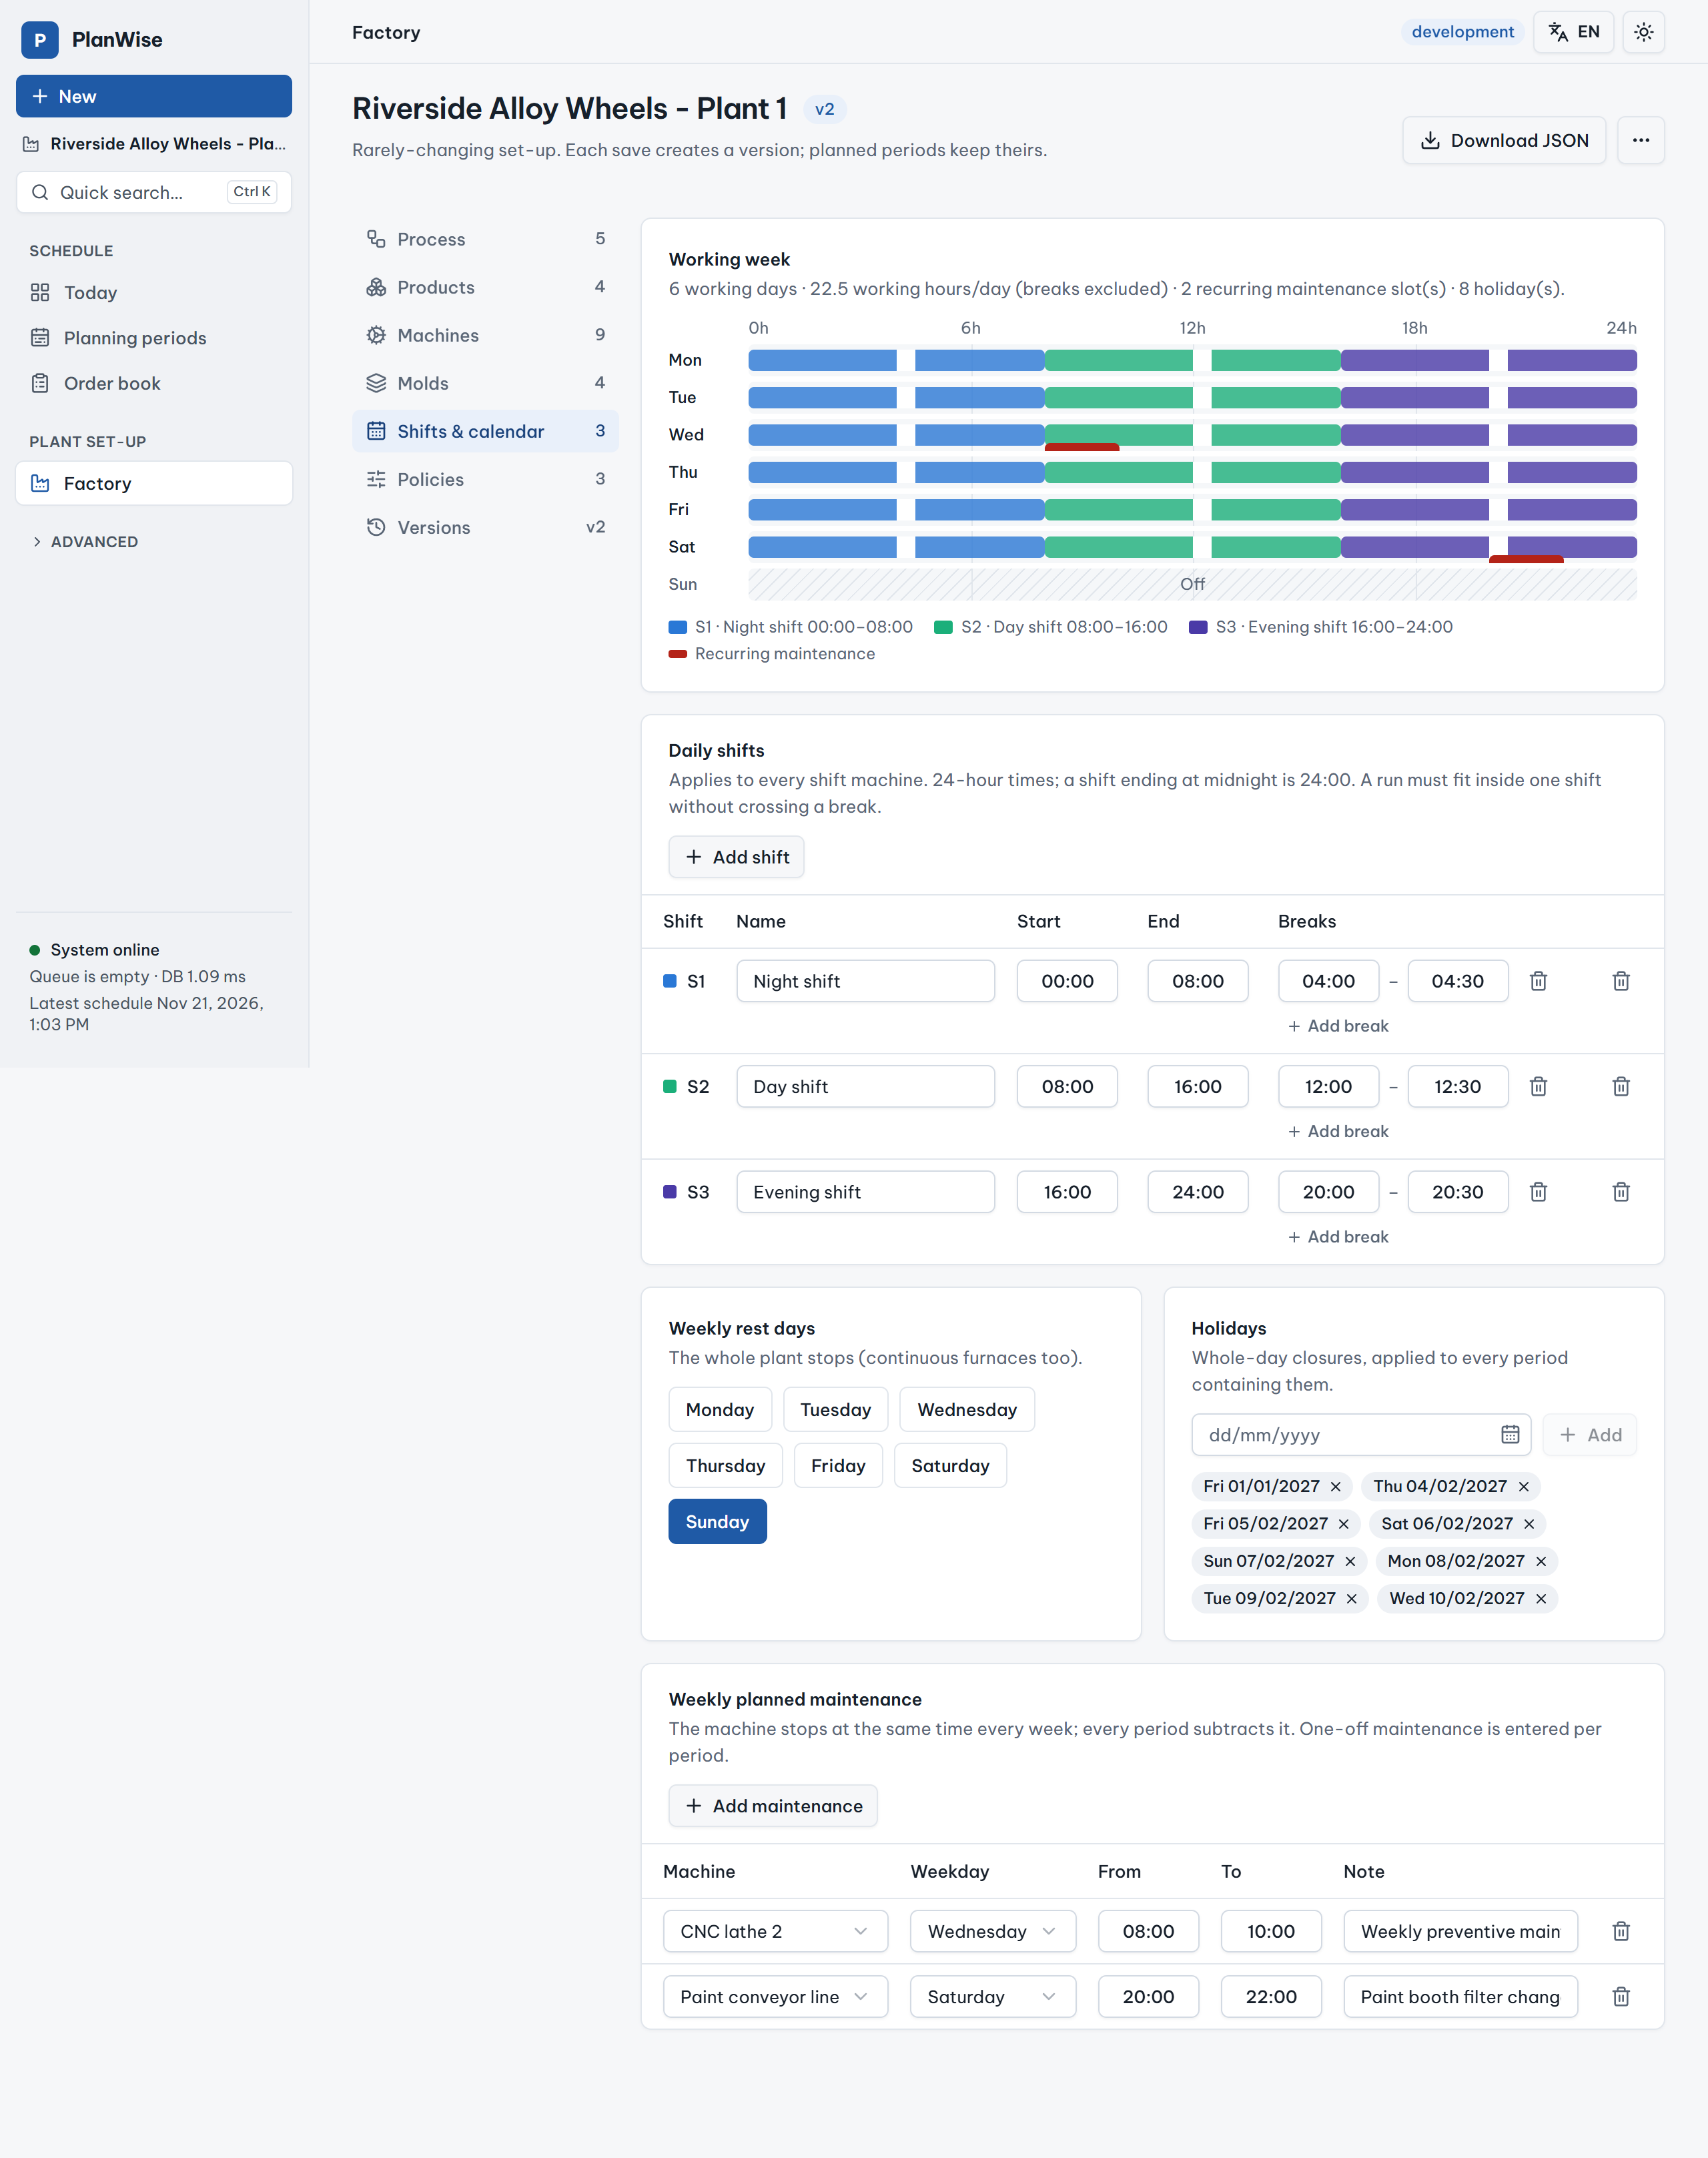
\includegraphics[width=0.62\linewidth]{factory_calendar}
\caption{Shifts \& calendar: week grid, daily shifts, rest days, holidays and weekly maintenance.}\label{fig:factory_calendar}
\end{figure}

\begin{description}[style=nextline, leftmargin=1.2em, font=\bfseries\color{brand}]
  \item[Working week grid] A visual summary of a week: shifts per day, breaks, rest days and recurring
        maintenance. Overlapping shifts are flagged.
  \item[Daily shifts] Apply to every machine on a shift calendar. Times are 24-hour; a shift ending at
        midnight ends at 24:00. Each shift can have breaks. \textbf{A run must fit inside one shift without
        crossing a break}, which is why breaks influence how long runs can be. The example uses three
        eight-hour shifts (night 00:00--08:00, day 08:00--16:00, evening 16:00--24:00) with a 30-minute meal
        break each.
  \item[Weekly rest days] The whole plant stops, continuous furnaces included (Sunday in the example).
  \item[Holidays] Whole-day closures, applied to every period that contains them (New Year and Lunar New
        Year in the example).
  \item[Weekly planned maintenance] A machine stops at the same time every week (weekday, from, to, note),
        and every period subtracts that time. One-off maintenance belongs to a period instead
        (Section~\ref{sec:period-calendar}).
\end{description}

\section{Policies}\label{sec:policies}

A policy decides which schedule counts as better. The score of a schedule is
\[ \text{score} = \sum_{\text{terms}} \text{weight} \times \text{objective value}, \qquad \text{lower is better}. \]
Terms marked \ui{Strictly first} are multiplied by a large scale factor (here one million) before summing, so
they always dominate the others: two schedules are first compared on those terms, and the others only break
ties. Each period picks one policy; the default is marked with a star.

\shot{factory_policies}{The default policy ``On-time delivery first'' with its weights.}{factory_policies}

For each objective term you set a \ui{Weight}; \ui{Share} shows its share of the total weight, and the
checkbox makes it strictly first (only possible with a weight above zero). \ui{Make default},
\ui{Duplicate} and delete are available per policy; the default policy cannot be deleted.

\begin{center}
\begin{tabularx}{\linewidth}{>{\bfseries}p{4.4cm}X}
\toprule
\rowcolor{white}Objective term & What is measured \\
\midrule
Weighted tardiness & Minutes late $\times$ order priority, summed over orders. \\
Safety-stock shortfall & Units below safety stock, summed over the end-of-day checkpoints. \\
Makespan & Minutes from the period start to the end of the last run. \\
Non-productive minutes & Minutes of opened machine shifts not spent processing (idle, setup, maintenance). \\
Setup minutes & Total changeover minutes between items. \\
Mold maintenance minutes & Total mold service minutes. \\
Idle minutes & Machine minutes left unused inside opened shifts. \\
Pulled-ahead units & Units made ahead for orders due after the period. \\
Pull-ahead options & Runs (options) made ahead for after-period orders. \\
Stock above safety & Units held above safety stock at the checkpoints. \\
Semi-finished left at end & Semi-finished units left at the end of the period. \\
\bottomrule
\end{tabularx}
\end{center}

The example plant has three policies: \textbf{On-time delivery first} (default; weighted tardiness and
safety-stock shortfall strictly first), \textbf{Balanced} (one weighted sum) and \textbf{Lowest running cost}
(for slack weeks: fewer shifts, setups and idle time; small delays tolerated).

\begin{note}
Weights belong to the factory. The \ui{Service first / Balanced / Cost first} switch on the Options tab
(Section~\ref{sec:ranking}) only changes the \emph{order} in which the same weighted terms are compared, not the
weights.
\end{note}

\section{Versions}\label{sec:factory-versions}

\shot{factory_versions}{Two versions: v2 (CNC lathe 3, effective 7 December) and v1 (imported).}{factory_versions}

Every save creates an immutable version. Each row shows the version number, \ui{latest}, the effective date,
when and by whom it was saved, the change note, how many periods use it, and the number of changes. Expand a
version to see its changes, then:

\begin{itemize}
  \item \ui{Compare with the current one} shows a side-by-side list: left the value in the old version, right
        the current value (including your unsaved draft);
  \item \ui{Restore into the draft} loads that version into the draft so you can review and save it as a new
        version.
\end{itemize}

\shot{factory_version_compare}{Comparing version 1 with the current set-up.}{factory_version_compare}

\begin{tip}
When a newer version becomes applicable to an existing period (for example you saved a version effective
from a date inside the period), the period header shows ``Factory set-up v\textit{N} available\dots''. Click it
and confirm \ui{Use v\textit{N}} to move the period to that version; its inputs are then checked again.
\end{tip}

\chapter{The order book}\label{ch:orders}

Orders are entered once, in the order book. Each planning period takes the open orders due in it; orders are
marked delivered when the period that delivered them is closed. You never type orders into a period by hand,
except for the rare period-only order (Section~\ref{sec:period-orders}).

\section{Page overview}

\shot{orders}{The order book with the expected load and the list of open orders.}{orders}

\begin{callouts}
  \item[1] \textbf{Expected load, next 8 weeks}: the open orders' demand per stage and week (below).
  \item[2] \textbf{Search} by order number, product or customer.
  \item[3] \textbf{Status filter}: Open (default), Delivered, Cancelled, or all; the \ui{\texttimes} clears it.
  \item[4] \textbf{Template}: downloads a CSV with the expected columns, in the interface language.
  \item[5] \textbf{Import from Excel}: imports an .xlsx/.csv file or pasted rows (Section~\ref{sec:import}).
  \item[6] \textbf{Add order}: enter a single order.
  \item[7] \textbf{Sortable columns}: click a header to sort, again to reverse.
\end{callouts}

\section{Expected load}

The panel converts the open orders' demand into machine-hours per stage, per week (using the fastest machine
and excluding setups), and compares it with the working calendar. A percentage above 85 is tight. Hover a
cell to see ``need / available machine-hours''. Above the table, two warnings may appear: how many open orders
are already overdue, and how many orders due within seven days are in no open period. Both are also shown
on the Today page.

\section{The order list}

Each row shows the order number, the product (with its colour dot), quantity, due date and time, priority,
customer and status. Overdue open orders are marked \ui{overdue}. The list is paged; the result count is
shown on the right.

\section{Adding, editing and deleting an order}

Click \ui{Add order}, or click an order number to edit it:

\shotf[0.5\linewidth]{order_dialog}{Editing an order.}{order_dialog}

\begin{center}
\begin{tabularx}{\linewidth}{>{\bfseries}p{3cm}X}
\toprule
\rowcolor{white}Field & Meaning \\
\midrule
Order code & Unique identifier (for example \code{SO-261124-039} or a customer PO). Fixed after creation. \\
Product & One of the factory's products. \\
Quantity & Units ordered (a whole number). \\
Due & Date and time the customer expects the goods (plant local time). \\
Priority & \ui{Low} (1), \ui{Normal} (2), \ui{High} (3), \ui{Urgent} (4). Lateness is weighted by priority, so an hour late on an urgent order costs four times an hour on a low one. \\
Pickup & \ui{At due time}: the customer collects at the due time, so goods finished early wait in the warehouse (and count against the stock cap). \ui{When ready}: the order ships as soon as it is finished. \\
Customer, Note & Free text, shown in periods and exports. \\
Status & \ui{Open}, \ui{Delivered} or \ui{Cancelled}. Closing a period sets delivered orders automatically; you rarely change it by hand. \\
\bottomrule
\end{tabularx}
\end{center}

Changes are saved to the book immediately. Open periods that use the order notice the change and offer to
take it in (Section~\ref{sec:sync}).

\begin{warning}
\ui{Delete} removes the order from the book completely, and periods using it are prompted to update. To keep
a record of an order the customer withdrew, set its status to \ui{Cancelled} instead.
\end{warning}

\section{Importing orders from Excel, CSV or a paste}\label{sec:import}

New orders usually arrive as a spreadsheet. The import reads it, shows a preview of every row with the
problems it found, and writes nothing until you confirm.

\shotf[0.82\linewidth]{import_start}{Step 1: choose a file or paste rows copied from Excel.}{import_start}

\begin{steps}[Import orders]
\begin{enumerate}
  \item Click \ui{Import from Excel} (also in the \ui{New} menu and on the Today page).
  \item Either \ui{Choose an .xlsx or .csv file} (the first sheet is read; the first row holds the headers),
        or copy rows from Excel, paste them in the text box and click \ui{Preview the pasted rows}.
  \item Read the preview (Figure~\ref{fig:import_preview}): the badges summarise what will happen, the
        \ui{Columns found} line shows how each header was understood, and each row has a result.
  \item Choose the mode, then click \ui{Write \textit{n} changes}.
\end{enumerate}
\end{steps}

\shotf[0.85\linewidth]{import_preview}{Step 2: the preview. Three new orders, one update of an existing order, one row with an unknown product.}{import_preview}

\subsection{How the file is read}

\begin{itemize}
  \item \textbf{Headers} may be English or Vietnamese, with or without accents, in any order: ``Order no'',
        ``PO'', ``Mã đơn'' all mean the order code; ``Qty'', ``Số lượng'' the quantity; and so on.
        Appendix~\ref{app:import} lists every accepted header. Unknown columns are ignored and named in
        the preview.
  \item \textbf{Required columns}: order code, product, quantity and due date. If one is missing, the preview
        says ``Missing required columns'' and nothing can be written.
  \item \textbf{Dates}: \code{dd/mm/yyyy} (also \code{dd-mm-yy} or \code{dd.mm.yyyy}), ISO
        \code{yyyy-mm-dd}, or real Excel dates. A time may follow the date or sit in its own column
        (\code{16:00}, \code{16h}); without a time, the factory's default due time is used.
  \item \textbf{Quantities} are whole numbers; \code{1.200} or \code{1,200} are read as twelve hundred.
  \item \textbf{Priority} may be a number 1--9 or a word: Low (Thấp), Normal (Thường), High (Cao), Urgent or
        Rush (Gấp).
  \item \textbf{Pickup} words: ``at due'', ``on due'', ``đúng hẹn'' for at due time; ``when ready'',
        ``ASAP'', ``khi xong'' for when ready.
  \item \textbf{Product} must be a product code; a close misspelling is suggested in the check notes.
\end{itemize}

\subsection{Row results}

\begin{center}
\begin{tabularx}{\linewidth}{>{\bfseries}p{2.4cm}X}
\toprule
\rowcolor{white}Result & Meaning \\
\midrule
Add & A new order code: it will be created. \\
Update & The code exists and is open; the check notes list what changes (for example ``changes: Quantity, Note''). \\
Same & The code exists with identical values; nothing to do. \\
Skip & The order is already delivered or cancelled; it is never changed by an import. \\
Error & The row cannot be used; the reason is shown in red (unknown product, bad date, missing quantity\dots). \\
\bottomrule
\end{tabularx}
\end{center}

If some rows have errors, writing is blocked until you either fix the file or tick \ui{Skip the \textit{n} rows
with errors and write the rest}.

\subsection{Import modes}

\begin{description}[style=nextline, leftmargin=1.2em, font=\bfseries\color{brand}]
  \item[Add \& update] (default) Orders in the file are added or updated; all other orders stay as they are.
        Use it for a file of new or changed orders.
  \item[Replace all open orders] Open orders missing from the file are \emph{cancelled}. Use it only when the
        file is the complete list of open orders (for example an export from the sales system). The preview
        shows how many open orders will be cancelled before you confirm.
\end{description}

\section{How orders reach planning periods}\label{sec:orders-periods}

\begin{itemize}
  \item When a period is created, it takes every \textbf{open} order due before its end --- including orders
        that are already overdue, which are scheduled as early as possible --- plus the open orders due in
        the look-ahead window after it (shown as ``after the period'').
  \item Changes made later in the book (new, changed or cancelled orders) are \emph{not} pushed into periods
        silently. The period's Prepare step shows a banner and you take them in with one click
        (Section~\ref{sec:sync}).
  \item An order becomes \ui{Delivered} when the period whose executed schedule delivers it is closed. Until
        then it stays open --- which is why a committed period should be closed before the next one is
        created (Section~\ref{sec:new-period}).
\end{itemize}

\chapter{Planning periods}\label{ch:periods}

A planning period is a window of days (usually two weeks) that is scheduled as one problem. It takes the
factory set-up and the open orders; you check its inputs, generate and commit a schedule, run it, and roll
over to the next period.

\section{The list of periods}

\shot{periods}{Planning periods: one open period (with its variant and reschedule) and one closed period.}{periods}

The page groups periods into \ui{Current \& upcoming} and \ui{Closed}. For each period you see its name and
dates, its status with the next step as a link, the number of orders inside and after it, the number of
options (and how many are still solving), the committed option and when it was committed, and the last
update. What-if variants and reschedules are listed under their main period. Click a period name to open
it; click the column headers to sort.

\subsection{Period statuses}\label{sec:statuses}

\begin{center}
\begin{tabularx}{\linewidth}{>{\bfseries}p{3.7cm}Xp{4.3cm}}
\toprule
\rowcolor{white}Status & Meaning & Next step shown \\
\midrule
Draft & Created, inputs not checked yet. & Check orders and opening stock \\
Inputs need fixing & The last save found errors; schedules cannot be generated. & Fix the errors under Prepare \\
Ready to schedule & Inputs are valid. & Generate schedule options \\
Solving & Runs are queued or running. & Wait for the solver \\
Options ready & At least one feasible schedule exists. & Compare and commit a schedule \\
Committed & An option has been committed. & Issue work orders, watch for incidents \\
Closed & The period is finished and read-only. & Period finished \\
\bottomrule
\end{tabularx}
\end{center}

A period whose end date has passed while it is still open is flagged \ui{Overdue to close}: its undelivered
orders are stuck in it until it is closed.

\section{Creating a period}\label{sec:new-period}

Click \ui{Plan a new period} (on this page, on Today, or in the \ui{New} menu). You only pick the dates; plant
set-up, shifts, rest days and open orders come in automatically.

\shotf[0.55\linewidth]{new_period}{Plan a new period. The warnings explain consequences before the period is created.}{new_period}

\begin{description}[style=nextline, leftmargin=1.2em, font=\bfseries\color{brand}]
  \item[Starts] Proposed as the day after the last period (``Right after Weeks 48-49''). A date in the past is
        allowed but flagged: the period would schedule past days.
  \item[Days] Defaults to the factory's period length. The resulting date range is shown below.
  \item[Name (optional)] Left empty, the period is named after its dates.
  \item[Opening stock] \ui{From the previous committed schedule}: finished goods, semi-finished stock and mold
        counters are projected from the closing state of the previous committed period, and you only correct
        what differs. \ui{Start from zero and enter counts}: for the very first period or after a stock-take.
  \item[Take open orders from the order book] Shows how many orders fall in the period and how many in the
        look-ahead window after it.
\end{description}

The dialog warns you about situations that usually indicate a mistake:

\begin{itemize}
  \item orders already due before the start --- they are taken into the period to ship as early as possible;
        consider telling the customers;
  \item the previous period is committed but not closed --- the orders it delivers are still open and would
        be taken again. Prefer opening it, going to Execute and using \ui{Close \& start the next period}
        (Section~\ref{sec:close}), which closes it and creates the next period in one step;
  \item the new period overlaps an open period --- allowed, but both may schedule the same orders.
\end{itemize}

Click \ui{Create period}. The period opens on its Prepare step.

\section{The period page}\label{sec:period-page}

\shot{period_header}{The period page of ``Weeks 48-49'' (here on the Prepare step).}{period_header}

\begin{callouts}
  \item[1] \textbf{Name and status.} Variants and reschedules add their label after the name and a kind badge
           (\ui{What-if variant}, \ui{Reschedule}).
  \item[2] \textbf{Key facts}: dates, length, orders in and after the period, and the factory set-up version
           the period uses (click it to open the Factory page). A reschedule also shows ``fixed before'' its
           cut-off.
  \item[3] \textbf{Versions of the period}: the main period and its reschedules and variants as chips; the
           committed one has a tick. Click a chip to switch (Chapter~\ref{ch:variants}).
  \item[4] \textbf{Next-step banner}: what to do now, with a button that goes there --- for example
           ``2 options are ready. Next: compare them and commit one.'' or, as here, ``Committed \dots\ Next:
           issue work orders, track incidents, and close the period at the end.''
  \item[5] \textbf{Step tabs}: Prepare, Options, Schedule \& compare, Commit, Execute. A green tick marks a done
           step, a number the current or a future step, a red dot a step with errors.
  \item[6] \textbf{Analysis and History}: how the scheduling went, and the change log (Chapter~\ref{ch:analysis}).
  \item[7] \textbf{More} and \textbf{Generate options}/\textbf{Generate more}.
\end{callouts}

\shotf[0.32\linewidth]{more_menu}{The \ui{More} menu of a period.}{more_menu}

The \ui{More} menu offers \ui{Create a what-if variant\dots} (Chapter~\ref{ch:variants}), \ui{Rename\dots}
and \ui{Delete period\dots} (for a variant or reschedule: \ui{Delete this version\dots}). Deleting removes
the inputs, options and decisions of that period or version and of its child variants and reschedules; the
order book is not affected.

\begin{note}
The tab you are on is part of the address (for example \code{?tab=schedule}), so you can bookmark a step or
send a colleague a link to it.
\end{note}

\chapter{Preparing a period}\label{ch:prepare}

The \ui{Prepare} step gathers everything that changes from one period to the next: the orders, the opening
stock, one-off machine stops, the policy and the pull-ahead choice. You edit them as one draft and save; the
backend then recompiles the period (lots, runs, machine availability) and reports in plain words anything
that is wrong.

\section{Input check and stage load}

\shotf[0.85\linewidth]{prepare_check}{The input check and the estimated stage load of the period.}{prepare_check}

\begin{itemize}
  \item \textbf{Input check} says ``Inputs are valid --- schedules can be generated'' or lists the errors and
        warnings. Errors block scheduling; warnings do not. Click an issue to jump to the section it concerns.
        Notes written by the system (for example ``Opening stock projected from the committed schedule of
        Weeks 46-47'') appear below.
  \item \textbf{Stage load} is the same estimate as on the Today page, but for this period only: machine time
        needed versus machine time available per stage, setups excluded.
\end{itemize}

Typical errors are a product without an eligible machine, opening stock above a store's capacity, a pull-ahead
quantity beyond the demand after the period, or a stage whose estimated load exceeds its capacity (``Stage
heat needs at least \dots\ machine minutes'').

\section{Orders}\label{sec:period-orders}

\shot{prepare_orders}{The Orders section: orders due in the period, with their source and allocation from stock.}{prepare_orders}

The section header summarises the demand per product. Two tables follow:

\begin{itemize}
  \item \textbf{Orders due in the period}: delivered inside the period. The scheduler tries to meet each due
        date, weighted by priority.
  \item \textbf{Orders after the period} (scroll down): due within the look-ahead window after the period.
        They are not delivered in it; they only matter for pulling work ahead (Section~\ref{sec:pull-ahead}).
\end{itemize}

The \ui{From stock} column is the quantity shipped straight from finished stock. \ui{auto} means the system
allocates stock above the safety level to the earliest orders. An order carried over from a reschedule keeps
what was already made for it (marked \ui{carried}).

Click the pencil of an order to change it for this period only --- for example raise its priority because the
customer called --- or the bin to remove it from this period:

\shotf[0.5\linewidth]{period_order_dialog}{Editing an order inside the period; the change applies to this period only.}{period_order_dialog}

\ui{Add a period-only order} creates an order that exists only in this period (marked \ui{period only}), for
example an internal replenishment. To change the original order or import more orders, use the order book.

\section{Taking in changes from the order book}\label{sec:sync}

When the order book changes after the period took its orders, a banner tells you how many orders are new,
changed or cancelled:

\shotf[0.95\linewidth]{prepare_sync}{The order book changed: one new order can be taken into the period.}{prepare_sync}

\ui{Update the period} takes the changes in: new orders are added, changed ones are refreshed (keeping your
\ui{From stock} choice), cancelled ones are removed. The button is disabled while you have unsaved edits ---
save or discard them first.

\begin{note}
For a reschedule, orders that were already delivered before its cut-off are left out on purpose; they are not
reported as new even though the order book still lists them as open until the period closes.
\end{note}

\section{Opening stock}\label{sec:opening}

\shot{prepare_opening}{Opening stock: actual versus projected finished goods, work in progress and mold counters.}{prepare_opening}

When the period was created from a previous committed schedule, every figure is projected from that
schedule's state at the end of the previous period (``Projected from the committed schedule up to \dots'').
Count the actual stock on the floor and correct only what differs: edited cells are highlighted and counted
(``2 corrected''). \ui{Reset to projection} undoes your corrections. If there was no earlier committed schedule,
enter the counts.

\begin{description}[style=nextline, leftmargin=1.2em, font=\bfseries\color{brand}]
  \item[Finished goods] Per product: \ui{Actual}, \ui{Projected}, \ui{Safety} and \ui{Cap}. Values below
        safety are flagged; the scheduler then plans production to catch up, and the shortfall counts at the
        checkpoints until it does.
  \item[Semi-finished (WIP)] Per semi-finished code, with its stage and store capacity.
  \item[Molds] Cycles used since the last maintenance, against the limit. A mold near its limit will be
        serviced early in the period.
\end{description}

\section{Machine calendar}\label{sec:period-calendar}

\shot{prepare_calendar}{The machine calendar of the period: one row per machine, one column per day.}{prepare_calendar}

The grid shows each machine for each day of the period. Hatched cells are plant rest days or holidays;
\textbf{B} marks maintenance (recurring from the factory set-up, or a period exception); \textbf{!} marks a
breakdown; faded cells lie before a reschedule's cut-off. Hover a cell to see the details. The daily shift
times are repeated above the grid.

To add a one-off stop, click the machine's cell on that day (or \ui{Add an exception}):

\shotf[0.5\linewidth]{exception_dialog}{A calendar exception: T6 batch furnace 1 stops on 2 December 08:00--16:00.}{exception_dialog}

Choose the \ui{Machine} (or \ui{Whole plant}), the \ui{Kind} (\ui{Maintenance}, \ui{Breakdown}, \ui{Closed},
\ui{Other}), \ui{From} and \ui{To} (start and end time) and an optional note, then \ui{Apply}. The exception
appears in the \ui{Period exceptions} table below the grid, where it can be edited or deleted.

\begin{tip}
Weekly maintenance and yearly holidays belong on the Factory page so that every period applies them
automatically. Use period exceptions for one-off events: an extra inspection, a planned repair, a Saturday off.
\end{tip}

\section{Policy and pull-ahead}\label{sec:pull-ahead}

\shot{prepare_policy}{Choosing the objective policy and the pull-ahead options of the period.}{prepare_policy}

\begin{description}[style=nextline, leftmargin=1.2em, font=\bfseries\color{brand}]
  \item[Objective policy] Pick one of the factory's policies (Section~\ref{sec:policies}). Each card shows
        which terms are strictly first and the main weights. The default is preselected.
  \item[Pull ahead for long-term orders] Lets idle capacity make part of the after-period orders early. For
        each product with demand after the period you may allow a number of finished lots (one run of the last
        stage each) and/or runs at earlier stages (for example casting runs). Each allowed lot or run is an
        \emph{option}: the solver only uses it when it pays off under the policy. You can never pull ahead more
        than the demand after the period; this is checked on save.
\end{description}

\section{Saving and checking}

As soon as you change anything, a bar appears at the bottom of the page:

\shotf[0.95\linewidth]{prepare_save_bar}{Unsaved changes in the Prepare step.}{prepare_save_bar}

\ui{Save \& check} sends the inputs to the backend, which recomputes lots and runs and checks everything; the
input check and status update immediately. \ui{Discard} drops your changes. If options already exist, they
are kept but marked as based on the old inputs, and a banner offers \ui{Generate options for the new inputs}.

\begin{warning}
If somebody else saved the same period while you were editing, the bar warns that saving will conflict.
Discard and redo your change on the new version; PlanWise never silently overwrites another person's edit.
\end{warning}

\chapter{Generating schedule options}\label{ch:generate}

Once the inputs are valid, PlanWise can generate schedule options. Each algorithm yields one feasible
schedule from the same data; the system then keeps the schedules that no other schedule beats on every axis,
for you to compare (Chapter~\ref{ch:options}).

\shot{options_empty}{A period without options yet (here a what-if variant).}{options_empty}

\section{The Generate dialog}

Click \ui{Generate the first options} (or \ui{Generate options} / \ui{Generate more} in the period header).
You choose \emph{how long to wait}, not which solver:

\shotf[0.62\linewidth]{generate_dialog}{Choosing the search effort.}{generate_dialog}

\begin{center}
\begin{tabularx}{\linewidth}{>{\bfseries}p{2.2cm}p{3.6cm}X}
\toprule
\rowcolor{white}Preset & Runs & When to use \\
\midrule
Quick & EDD rule + Hybrid, 60~s & About a minute --- enough to see where things stand and how many orders are late. Good for a first look or a what-if variant. \\
Balanced & EDD rule + Hybrid, 180~s & Recommended for a two-week period; about three minutes. \\
Thorough & EDD rule + Hybrid, 600~s & Cuts operating cost further when there is time; about ten minutes. \\
\bottomrule
\end{tabularx}
\end{center}

The earliest-due-date rule (EDD) finishes in well under a second and is always included as a yardstick: an
optimised schedule must beat it to be worth the wait. The \term{Hybrid} method does the real work within the
budget, in three steps: dispatching rules give a fallback schedule; simulated annealing runs several seeds in
parallel to bring late orders down; then CP-SAT starts from the best schedule found to cut operating cost.
Each step replaces the previous result only when it is better, and it uses every processor core.

The footer shows how many runs will be queued and an upper bound of the waiting time. \ui{Generate
\textit{n} options} queues them.

\section{Customising algorithms, seeds and budget}

\ui{Customise algorithms, seeds and budget\dots} reveals every algorithm, grouped by family:

\shotf[0.6\linewidth]{generate_custom}{Custom selection of algorithms.}{generate_custom}

\begin{longtable}{>{\bfseries}p{3.5cm}p{2.4cm}p{8.6cm}}
\toprule
\rowcolor{white}Algorithm & Family & How it works \\
\midrule
\endhead
FIFO & Dispatching rule & First in, first out: at each step pick the operation that can start earliest; ties follow list order. \\
EDD & Dispatching rule & Earliest due date: as FIFO, ties favour the order due soonest. \\
SPT & Dispatching rule & Shortest processing time: as FIFO, ties favour the shortest run. \\
Simulated Annealing & Metaheuristic & Searches the priority order and machine choice, building schedules with the same decoder as the rules; accepts worse moves under a cooling temperature to escape local optima. \\
Genetic Algorithm & Metaheuristic & A population of solutions with tournament selection, crossover, mutation and elitism; schedules built with the same decoder. \\
CP-SAT & Constraint programming & One monolithic constraint model without hints: chooses machines, shifts, sequence and build-ahead options on its own. Needs a long budget on a two-week period. \\
CP-SAT + EDD hint & Constraint programming & CP-SAT warm-started from the EDD schedule; if it cannot improve, the EDD schedule is kept. \\
CP-LNS & Constraint programming & Large neighbourhood search: starts from the best rule schedule; each round reopens a time window, a few machines or one stage for CP-SAT to re-sequence. \\
Hybrid: search, then CP-SAT & Constraint programming & The three-step method described above; recommended for two-week periods. \\
Rolling-horizon CP-SAT & Constraint programming & Splits the horizon into consecutive windows, solves each with CP-SAT and freezes what is already scheduled. \\
\bottomrule
\end{longtable}

\begin{description}[style=nextline, leftmargin=1.2em, font=\bfseries\color{brand}]
  \item[Seeds for randomised algorithms] 1--3. The metaheuristics and CP-SAT searches are randomised; running
        two or three seeds gives a better chance and shows how stable the result is. Rules run once.
  \item[Budget per run (seconds)] The time limit of each non-rule run, up to the maximum published by the
        backend (900~s by default). A warning appears when CP-SAT gets less than two minutes: that is usually
        too short to improve a two-week schedule, so it will keep the EDD schedule.
\end{description}

\begin{note}
The dialog only offers algorithms the backend supports for the period's model. Hybrid and rolling-horizon
CP-SAT exist for the five-stage model only; for four-stage JSON scenarios (Advanced) the presets use rules,
simulated annealing, a genetic algorithm, CP-SAT with hint and CP-LNS instead.
\end{note}

\section{While the solver works}

Runs are queued and solved in the background on the server. You can keep working, open other pages or
close the browser. The period status becomes \ui{Solving}, the header shows ``Solving \textit{n} options
(Hybrid). The page updates when they finish.'', and the Options tab shows a spinner. When a run finishes, its
schedule is first checked by an \textbf{independent validator}; only valid schedules become options. The
page then updates on its own.

Each run ends with a solver status:

\begin{center}
\begin{tabularx}{\linewidth}{>{\bfseries}p{5.6cm}X}
\toprule
\rowcolor{white}Status & Meaning \\
\midrule
Feasible schedule & A valid schedule; not proven optimal (normal within a time limit). \\
Optimal & CP-SAT proved no better schedule exists for this model. \\
No improvement found, EDD schedule kept & A CP-SAT method ran out of time before improving the starting schedule. \\
No feasible schedule & The algorithm could not place everything; check the inputs (capacity, calendar). \\
\bottomrule
\end{tabularx}
\end{center}

\begin{tip}
If the analysis says ``The optimiser found nothing better than the dispatching rules'', it offers
\ui{Generate with Thorough}: the search and CP-SAT then get about ten minutes.
\end{tip}

\chapter{Comparing options and ranking}\label{ch:options}

The \ui{Options} tab shows the schedules worth considering, ranked under the period's policy. Its job is to
make the decision quick: most of the time, one of the first two cards is the schedule you will commit.

\shot{options}{The Options tab of ``Weeks 48-49'' with two recommended options.}{options}

\begin{callouts}
  \item[1] \textbf{What matters most this period?} The ranking policy: \ui{Service first}, \ui{Balanced} or
           \ui{Cost first} (Section~\ref{sec:ranking}).
  \item[2] \textbf{How this policy scores schedules}: opens the exact scoring rule.
  \item[3] \textbf{Recommended option cards}, ranked \#1, \#2, \dots\ under the selected policy.
  \item[4] \textbf{What really differs}: one sentence on where the recommended options are practically equal
           and where they really differ --- often the fastest way to decide.
  \item[5] \textbf{Viewing bar}: the option currently selected, its key figures, and \ui{Commit option}. It
           stays at the bottom of the screen on every tab.
\end{callouts}

\section{Which schedules are recommended}\label{sec:recommended}

Every schedule is placed on three axes:

\begin{enumerate}
  \item \textbf{priority-weighted lateness} (minutes late $\times$ priority, summed over orders);
  \item \textbf{safety-stock shortfall} (units below safety, summed over end-of-day checkpoints);
  \item \textbf{operating cost} (the weighted sum of all other policy terms: shifts, setups, idle time,
        maintenance, surplus stock, \dots).
\end{enumerate}

A schedule is \emph{dominated} when another schedule is at least as good on all three axes and better on one.
PlanWise recommends only the schedules that are \textbf{not} dominated: every other schedule is beaten by a
recommended one on all three axes. Dominated schedules are not hidden --- they appear in the Analysis tab and
in the \ui{Compare with} list --- but there is no reason to commit one.

Recommended options are named after what they are best at:

\begin{center}
\begin{tabularx}{\linewidth}{>{\bfseries}p{4.2cm}X}
\toprule
\rowcolor{white}Name & Meaning \\
\midrule
Best on every axis & Only one schedule is recommended: it is at least as good as every other on all axes. \\
Protects priority orders & Lowest priority-weighted lateness. It may still have more raw hours late, but on low-priority orders. \\
Least shortfall & Lowest safety-stock shortfall. \\
Lowest cost & Lowest operating cost. \\
Middle ground & Recommended without being best on any single axis --- a compromise. \\
\bottomrule
\end{tabularx}
\end{center}

Names combine when an option wins several axes (``Least shortfall · Lowest cost''). Each card shows who built
it (\ui{Built by: Hybrid: search, then CP-SAT}, \ui{Manual edit}, \ui{Optimised around an edit}), the four
headline figures (green = best among the recommended options), a one-line comparison with \#1, and badges such
as \ui{Committed} and \ui{Viewing}. Click a card for a \ui{Quick look} at the schedule, or to make it the
viewed option.

If you edited schedules by hand and an edit is not recommended, it is listed under \ui{Your versions not
recommended} with the reason, so your work never disappears.

\section{Ranking policies}\label{sec:ranking}

The recommended options are ordered by a score. The switch at the top picks how the weighted terms of the
factory policy are combined:

\begin{description}[style=nextline, leftmargin=1.2em, font=\bfseries\color{brand}]
  \item[Service first] (default) Lateness and safety-stock shortfall are compared first (tier~1); operating
        cost only breaks ties (tier~2). A score reads ``tier~1 · tier~2''.
  \item[Balanced] Every weighted term is added into one score: trades a little safety stock or lateness for
        lower cost when the weights allow it.
  \item[Cost first] Operating cost is compared first; lateness and shortfall only break ties. Use it in slack
        weeks when orders can slip.
\end{description}

Switching re-ranks the same schedules instantly; nothing is recomputed. \ui{How this policy scores
schedules} shows the formula with the actual weights:

\shotf[0.82\linewidth]{options_scoring}{The scoring rule of ``Service first'' with the weights of the factory policy.}{options_scoring}

\begin{note}
The weights come from the factory's policy (Section~\ref{sec:policies}). This switch only changes the priority
order of the terms, not the weights. To change the weights, edit the policy on the Factory page or pick
another policy under Prepare.
\end{note}

\section{The trade-off chart}

Below the cards, a scatter plot places every schedule by operating cost (horizontal) and safety-stock
shortfall (vertical). Closer to the bottom-left corner is better. Named green dots are recommended options,
grey dots are other schedules, and a dashed line joins the recommended options.

\shotf[0.8\linewidth]{options_tradeoff}{Trade-off between operating cost and safety-stock shortfall.}{options_tradeoff}

\section{Key figures used everywhere}\label{sec:kpis}

The same figures appear on the cards, in the Schedule \& compare tiles, in the viewing bar and in exports:

\begin{longtable}{>{\bfseries}p{4.1cm}p{10.4cm}}
\toprule
\rowcolor{white}Figure & Definition \\
\midrule
\endhead
On time & Orders delivered by their due date, out of the orders of the period (for example 40/44). \\
Total lateness & Hours late summed over all late orders. \\
Priority-weighted lateness & Minutes late $\times$ order priority, summed (the policy's ``weighted tardiness''). \\
Safety-stock shortfall & Units below safety stock, summed over the end-of-day checkpoints. \\
Operating cost & Weighted sum of the non-service terms of the policy: non-productive time, setup, mold maintenance, makespan, surplus stock, pull-ahead, semi-finished left at the end. A relative figure for comparing schedules, not money. \\
Machine shifts open & Number of machine-shifts the schedule uses. Fewer shifts mean fewer people and less energy. \\
Idle time & Available minutes left unused inside opened shifts. \\
Setup & Changeover minutes on machines. \\
Mold maintenance & Mold service minutes. \\
Last required lot done & When the last lot needed by an order of the period leaves test and packing. \\
\bottomrule
\end{longtable}

\chapter{Schedule \& compare}\label{ch:schedule}

\ui{Schedule \& compare} shows one option in full detail: its figures, a Gantt chart of every run on every
machine, the deliveries, and --- when you pick a second option --- exactly what changes between the two.

\shot{schedule}{Schedule \& compare for the recommended option of ``Weeks 48-49''.}{schedule}

\begin{callouts}
  \item[1] \textbf{Option}: the schedule being viewed (recommended options first, then the others).
  \item[2] \textbf{Compare with}: a second option to compare against, or \ui{no comparison}.
  \item[3] \textbf{Edit this schedule by hand} (Chapter~\ref{ch:editing}). Next to it: which algorithm built the
           option, the solver status and when it ran.
  \item[4] \textbf{Figure tiles}: on time, total lateness, safety-stock shortfall, operating cost; \ui{4 more
           figures} adds machine shifts open, idle time, setup and last required lot done.
  \item[5] \textbf{View}: \ui{By machine} (Gantt), \ui{By order} (with the number of late orders), \ui{Machine
           load}.
  \item[6] \textbf{Colour by}: \ui{Product}, \ui{Lateness} or \ui{Priority}.
  \item[7] \textbf{Zoom}: \ui{Fit} (whole period on one screen), \ui{Days}, \ui{Shifts}, \ui{Hours}. Your zoom
           and colour choices are remembered in this browser.
  \item[8] \textbf{Legend}, ending with the red diamond for a late delivery.
\end{callouts}

\section{Reading the Gantt chart}\label{sec:gantt}

Each row is a machine, labelled with its code, stage and utilisation over the period (busy time including
setup and maintenance, divided by rostered time). Time runs left to right; vertical lines separate days and
a red \ui{Now} line marks the current time when it falls inside the period.

\begin{itemize}
  \item \textbf{Bars} are production runs. Furnace runs show their run number (01, 02, \dots). Bars in two
        colours mark semi-finished stock shared by a product line (front or rear).
  \item \textbf{Grey parts} of a bar are setup (changeover) and hatched parts are mold maintenance.
  \item \textbf{Pale blue bands} behind the bars are the shifts the schedule opens. A shift is only opened when
        a run needs it, which is how the schedule saves labour.
  \item \textbf{Hatched beige columns} are rest days and holidays; machines on a 24/7 calendar have a
        continuous band.
  \item \textbf{The Deliveries row} at the bottom marks each order's delivery: green when on time, a red
        diamond when late.
\end{itemize}

Hover a bar to see its details: run code, item, quantity, machine, shift, mold, start and end, setup time and
the orders it serves. Click a bar to highlight its whole product line across stages; click a delivery to see
the runs that feed that order. The arrow keys \kbd{\textleftarrow}\,\kbd{\textrightarrow} move between runs,
and \kbd{?} lists all shortcuts.

\shot{gantt_shifts}{Zoom \ui{Shifts}: individual shifts become visible; the tooltip details one casting run.}{gantt_shifts}

\subsection{Colour modes}

\begin{description}[style=nextline, leftmargin=1.2em, font=\bfseries\color{brand}]
  \item[Product] Silver and black, front and rear in different colours (the default).
  \item[Lateness] Red: the run feeds a late order; green: it feeds on-time orders; grey: not tied to an order
        (build-ahead or reserve). This is the quickest way to see where lateness comes from.
  \item[Priority] Shades from low to high priority of the orders a run serves.
\end{description}

\shot[0.92\linewidth]{gantt_lateness}{Colour by lateness: red runs feed late orders.}{gantt_lateness}

\section{Comparing two options}\label{sec:compare}

Pick an option under \ui{Compare with}. The Gantt chart then shows, for the viewed option, which shifts are
open only in this schedule or only in the compared one, and (with \ui{Show positions in the compared option})
dashed outlines where each run sits in the other schedule. The legend counts how many runs differ.

\shot{compare_gantt}{Comparing the recommended option with the EDD rule.}{compare_gantt}

Below the chart, a table answers ``Switching from A to B: what you gain and lose'' metric by metric: ranking,
late orders, total and priority-weighted lateness, shortfall, operating cost, machine shifts, idle time,
setup, mold maintenance and last lot done, each marked \ui{better}, \ui{worse} or \ui{equal}. It also lists
the shifts open only in one of the two schedules and how many shared runs moved.

\shotf[0.85\linewidth]{compare_diff}{What changes when switching from the recommended option to the EDD rule.}{compare_diff}

\begin{tip}
Comparing with the EDD rule is a good sanity check: it shows how much the optimiser actually gained (in the
example: nine fewer late orders and about 785 fewer hours late).
\end{tip}

\section{The order view and ``why is this order late?''}\label{sec:why-late}

\ui{By order} draws one row per order: a pale band from release to due date, a thick tick at the due date,
and coloured bars for the runs that feed it at each stage. Tick \ui{Late orders first} to sort the late ones to
the top; the right column says ``late 27.5~h'' or ``on time''.

\shot{by_order}{The order view with late orders first.}{by_order}

Click an order to open its explanation:

\shotf[0.9\linewidth]{why_late}{Why order SO-261126-051 is 27.5 hours late.}{why_late}

PlanWise looks for the causes a planner can act on and states them in plain sentences:

\begin{itemize}
  \item \textbf{Longest wait} at a stage between material ready and start, and why: the machine was busy with
        other runs (named), part of the wait fell outside open shifts, or shifts of that machine stayed closed
        during the wait --- in which case opening one or moving the run to another machine may cut the delay.
  \item \textbf{Bottleneck}: how much of its shift time the stage used while the order was open (``Heat
        treatment uses 100\% of its shift time \dots\ the bottleneck this order competes for'').
  \item \textbf{Competition}: runs of orders due later that went first at the last stage.
  \item \textbf{Physics}: the order was released so late that its supply chain alone takes longer than the time
        to its due date.
\end{itemize}

The table \ui{Supply chain of the lot that finished last} lists, stage by stage, the run, machine, start and
end, and how long the material waited before it (long waits in red). \ui{Edit by hand} opens the editor
directly from here.

\begin{note}
In the five-stage model, semi-finished stock is not pegged to orders: each step takes the latest run of the
needed item that finished before the next step started. The explanation points at where to act; it is not a
constraint the solver used.
\end{note}

\section{Machine load}

\ui{Machine load} shows, per machine and day, the share of rostered time the machine is busy (setup and
maintenance included). Orange cells ($\geq$ 90\%) are nearly full --- bottlenecks. A dash means the machine
does not work that day.

\shotf[0.9\linewidth]{machine_load}{Machine load by day: both furnaces are full for most of the period.}{machine_load}

\section{Deliveries and closing stock}

Further down the tab, two tables complete the picture:

\shotf[0.85\linewidth]{deliveries}{Deliveries: every order with its delivery time and slack or lateness.}{deliveries}

\ui{Deliveries} lists every order with product, quantity, delivery time, due time and its slack (positive) or
lateness. Filter \ui{All} or \ui{Late}, sort \ui{Most late first} or \ui{By due date}; click an order to see
its runs on the Gantt chart and the explanation above.

\shotf[0.85\linewidth]{closing_stock}{Closing finished-goods stock against the safety level.}{closing_stock}

\ui{Closing finished-goods stock} compares opening and closing stock per product with its safety level. Safety
stock is measured at every end-of-day checkpoint; this table shows the final one, and the tick on each bar
marks the safety level.

\chapter{Editing a schedule by hand}\label{ch:editing}

Planners know things the solver does not: a machine that is about to be serviced, a customer who called, a
team that would rather work one long run than two short ones. PlanWise lets you change any option directly.
\textbf{You decide the machine and the order of runs; the computer works out the times}, re-checks the whole
schedule and scores it, after every single change. The original option is never modified: your edit is saved
as a new option.

\section{Starting the editor}

On \ui{Schedule \& compare}, pick the option to start from and click \ui{Edit this schedule by hand} (or
\ui{Edit by hand} in an order's explanation, or \ui{Edit} in a quick look). Editing is available for
five-stage schedules of open periods.

\shot{editor_start}{The editor before any change: the toolbar, the figures ``as original'' and the Gantt chart.}{editor_start}

The editor shows a sticky toolbar, the five headline figures with their difference from the original, the
Gantt chart and, on the right, how to edit (until you select a run).

\section{Changing runs}\label{sec:edit-runs}

There are two ways to change a run:

\begin{itemize}
  \item \textbf{Drag} a bar to another machine of the same stage or to another time (in 15-minute steps). If
        the target machine cannot make that item, the bar turns red and cannot be dropped there.
  \item \textbf{Select} a bar (click it, or move to it with the arrow keys and press \kbd{Enter}) and use the
        run panel:
\end{itemize}

\shotf[0.72\linewidth]{editor_runpanel}{The run panel of a machining run moved from CNC\_1 to CNC\_2.}{editor_runpanel}

\begin{description}[style=nextline, leftmargin=1.2em, font=\bfseries\color{brand}]
  \item[Lock this run (L)] Keeps the run exactly as it is when you later use \ui{Optimise the rest}.
  \item[Original] Where the run was in the original option.
  \item[Machine] Move the run to another eligible machine. If only one machine can make it, the field says so.
  \item[Order on the machine] \ui{Earlier} / \ui{Later} swap it with the neighbouring run on its machine
        (``Run 5 of 29 on CNC\_2'').
  \item[Not before] An earliest start: the run starts at the earliest valid slot from that time. \ui{Not
        earlier than now} pins it to its current start; \ui{Clear} removes the constraint.
\end{description}

\section{Seeing the effect immediately}

\shot{editor}{After moving one run: the edit is valid, 60 cost units cheaper but 2.9 hours more late in total.}{editor}

\begin{callouts}
  \item[1] \textbf{Undo, redo, reset} (\kbd{Ctrl}\,\kbd{Z}, \kbd{Ctrl}\,\kbd{Shift}\,\kbd{Z}). Every change can be
           undone.
  \item[2] \textbf{How times are rebuilt}: \ui{Keep other times} (untouched runs keep their time; only runs that
           get pushed move) or \ui{Pack early} (every run starts as early as the current order allows).
  \item[3] \textbf{Exit}: leave the editor; unsaved changes are discarded after a confirmation.
  \item[4] \textbf{Optimise the rest\dots}: let CP-SAT re-sequence everything you did not lock.
  \item[5] \textbf{Save as new option}.
  \item[6] \textbf{Impact}: each figure with its change versus the original (green better, amber worse). The
           toolbar repeats it in one line, for example ``Valid · Late +2.9 h · Cost −60''.
  \item[7] \textbf{Run panel} of the selected run.
\end{callouts}

After every change the backend rebuilds the times (respecting shifts, setups, mold cycles and maintenance,
semi-finished stock and warehouse caps), runs the independent validator and scores the result. Changed runs
get a dashed outline, and a \ui{Changes} panel lists your edits and every run that moved as a consequence. A
banner explains shift effects (``The edit closes 1 shift(s): CNC\_1 16:00--00:00 Mon, 11/23. Operating cost
down 1,446.'').

If the edit breaks a rule, it cannot be saved and the problem is explained:

\begin{center}
\begin{tabularx}{\linewidth}{>{\bfseries}p{3.4cm}X}
\toprule
\rowcolor{white}Problem & Example message \\
\midrule
Warehouse full & Finished stock of F silver exceeds the warehouse cap at \dots \\
Material missing & Semi-finished F\_HEAT runs out at \dots: a run uses it before it is made. \\
Buffer full & Semi-finished buffer F\_CAST exceeds its capacity at \dots \\
Cannot ship & Not enough R black to ship at \dots \\
Beyond the period & Run \dots\ is pushed past the end of the period. \\
No slot & Cannot place \dots: they wait for semi-finished stock not made before them, or the period is full. Try moving the upstream run earlier. \\
\bottomrule
\end{tabularx}
\end{center}

Click \ui{Show} next to a problem to select the run concerned, then undo or keep editing until the schedule is
valid again.

\section{Optimise the rest}\label{sec:optimise-rest}

Often you only care about a few runs. Lock them (or simply edit them) and let CP-SAT re-sequence everything else:

\shotf[0.55\linewidth]{optimize_dialog}{Optimise the rest: 1 run kept, 296 runs CP-SAT may change.}{optimize_dialog}

\begin{description}[style=nextline, leftmargin=1.2em, font=\bfseries\color{brand}]
  \item[Kept / CP-SAT may change] How many runs stay fixed and how many may move.
  \item[Keep the runs I edited] On by default; locked runs are always kept.
  \item[Frozen zone] Runs starting before this point stay: \ui{None}, \ui{Until now} (while the period is
        running), \ui{First 24 h}, \ui{First 48 h} or \ui{Until\dots} a chosen time. Use it to leave the shifts
        already handed to the floor untouched.
  \item[Time allowed] 30~s, 2~min or 5~min. Longer usually finds more; you can keep working meanwhile.
  \item[Short name] Optional name of the resulting option.
  \item[Also save the current edit as its own option] To compare your hand edit with the optimised result.
\end{description}

The optimisation runs in the background like any solver run. Its result is a new option that is \emph{never
worse} than your edit; when it finishes a message says whether something better was found. With spare
capacity, CP-SAT may add build-ahead runs for long-dated orders to reduce safety-stock shortfall.

\section{Saving the edit}

\shotf[0.5\linewidth]{save_option_dialog}{Save as a new option.}{save_option_dialog}

Give the edit a short name (``Machining run moved to CNC lathe 2'') and, optionally, why you made it. The
original option is kept. The edit is ranked with the other options under the same policy and can be compared
and committed as usual; its card says \ui{Manual edit} and from which option it was made. A hand edit that
turns out to be the best schedule is recommended like any other --- in the example the edit became the
``Lowest cost'' option and was committed.

\chapter{Committing and executing}\label{ch:execute}

\section{Committing a schedule}\label{sec:commit}

When you are satisfied with an option, commit it. Committing says ``this is the plan''; work orders are
issued from the committed schedule, and its projected closing stock becomes the next period's opening stock.
Open the \ui{Commit} tab, or click \ui{Commit option} in the viewing bar.

\shot{commit}{The Commit tab: the option being committed, the mandatory reason and the decision log.}{commit}

\begin{steps}[Commit an option]
\begin{enumerate}
  \item Check \ui{You are committing}: the option's name and builder, on-time count, lateness, shortfall and
        the ranking policy. \ui{Change option} goes back to pick another one.
  \item Type the \ui{Reason} (required). It should say why this option and not another, for example ``accept
        3 extra shifts to keep enough F silver safety stock for long-dated orders''.
  \item Click \ui{Commit this option}. The status becomes \ui{Committed} and the next-step banner points to
        Execute.
\end{enumerate}
\end{steps}

The \textbf{decision log} below is stored on the server and is append-only: entries are never edited or
deleted. Each commit keeps the run, the data snapshot, the policy, the figures at that moment (late orders,
shortfall, machine shifts), the reason and who committed. You may commit another option until the period is
closed (\ui{Commit again}); the new row supersedes the previous one, and both remain visible.

\begin{note}
A decision must be explainable: the button refuses an empty reason (``Enter a reason before committing ---
the decision must be explainable''). If the server cannot be reached, the reason stays in the box so you can
try again.
\end{note}

\section{Work orders}\label{sec:work-orders}

The \ui{Execute} tab turns the committed schedule into work orders: what each machine does and when.

\shot{work_orders}{Work orders of Monday 23 November for all machines.}{work_orders}

\begin{itemize}
  \item Filter by \ui{Day} (or \ui{Whole period}) and by \ui{Machine} (or \ui{All machines}); the number of runs
        is shown.
  \item Each row gives the day and shift, the machine and stage, the run time, the run code and item, the
        quantity, and the preparation (when the changeover starts and how long it takes, the mold used, and a
        \ui{mold service} badge when maintenance precedes the run).
  \item \ui{CSV} exports the selection for Excel (with day, shift, machine, prep start, start, end, run, item,
        quantity, prep minutes and mold).
  \item \ui{Print} opens a printable sheet for the shift supervisors with a \ui{Done} column to tick and
        \ui{Prepared by} / \ui{Supervisor} signature lines.
\end{itemize}

If the period's inputs were changed after the commit, a banner warns that the work orders still follow the
committed schedule: if the change is real, generate new options and commit again.

\section{Incidents: replanning the rest of the period}\label{sec:incident}

When something goes wrong --- a machine breaks down, a rush order arrives, material is late --- you replan only
what has not happened yet. The \ui{An incident? Replan the rest} panel sits below the work orders:

\shot{incident_close}{Left: replanning after an incident. Right: finishing the period.}{incident_close}

\begin{steps}[Replan after a breakdown]
\begin{enumerate}
  \item Set the \ui{Cut-off}: the moment from which the plan changes (inside the period).
  \item Optionally choose the \ui{Machine down}, when it is \ui{Expected back} and \ui{What happened}. Leave
        \ui{None --- just replan} to replan without a breakdown (for example to add a rush order).
  \item Read the hint, which describes the state at the cut-off, for example ``By 30/11 08:00: 227/297 runs
        started, 21 orders delivered; still running on HT\_1 (until 16:00), HT\_2 (until 16:00)''.
  \item Click \ui{Replan from the cut-off}.
\end{enumerate}
\end{steps}

PlanWise creates a \term{reschedule} version of the period and opens its Prepare step:

\begin{itemize}
  \item what ran before the cut-off stays as it was (``fixed before'' the cut-off);
  \item runs in progress at the cut-off count as done, and their machine stays busy until they end;
  \item stock, molds and delivered orders are taken as of the cut-off; delivered orders leave the reschedule;
  \item the breakdown is entered as a calendar exception of the reschedule;
  \item pull-ahead is switched off (turn it back on under Policy if needed), so nothing is made ahead twice.
\end{itemize}

You can still adjust the reschedule (add a rush order, another stop), then generate options and commit as
usual. Section~\ref{sec:family} shows how reschedules appear among the versions of a period.

\section{Finishing the period}\label{sec:close}

The \ui{Finish the period} panel (right in Figure~\ref{fig:incident_close}) shows the projected closing stock
of each product against its safety level and how many orders the committed schedule delivers.

\begin{description}[style=nextline, leftmargin=1.2em, font=\bfseries\color{brand}]
  \item[Close only] Closes the period.
  \item[Close \& start the next period] Closes the period and creates the next one in one step, starting the
        day after with the projected closing stock as its opening stock. This is the normal end of a cycle.
\end{description}

Closing makes the period --- with its variants and reschedules --- read-only. The schedule that was executed
(the latest committed reschedule if there is one, otherwise the committed schedule of the period or variant)
is treated as what happened: the orders it delivered, including those delivered before each cut-off, are
marked \ui{Delivered} in the order book. Undelivered orders stay open and are picked up by the next period.

\shot{closed_period}{A closed period remains available for reference: its work orders, schedule, analysis and history.}{closed_period}

\begin{warning}
Close each period when it ends. A period that ended but is still open is flagged \ui{Overdue to close}, and the
orders it delivered remain open in the book, so a new period would take them again.
\end{warning}

\chapter{What-if variants and versions of a period}\label{ch:variants}

A period can have several \term{versions}: the main period, what-if variants and reschedules. They share the
period's dates and set-up but have their own inputs, options and decisions.

\section{What-if variants}

A variant is a copy of a version's inputs, used to answer ``what if\dots'' without touching the main plan:
what if we accept this rush order, open on Sunday, keep furnace~2 down for a day, or use another policy?

\begin{steps}[Create and use a variant]
\begin{enumerate}
  \item On the period page, open \ui{More} $\rightarrow$ \ui{Create a what-if variant\dots}.
  \item Give it a name (``Rush order from the export customer'', ``Open Sundays'') and click \ui{Create
        variant}. The variant opens on its Prepare step.
  \item Change what you want to test (add a period-only order, add a calendar exception, pick another policy),
        then \ui{Save \& check}.
  \item Generate options (\ui{Quick} is usually enough for a what-if) and compare them with the main period's
        options.
  \item If the variant is the better plan, commit one of its options. Whichever version is committed becomes
        the plan.
\end{enumerate}
\end{steps}

\shotf[0.5\linewidth]{variant_dialog}{Creating a what-if variant.}{variant_dialog}

\section{The family of versions}\label{sec:family}

All versions of a period appear as chips under the period header: \ui{Main}, then each reschedule (with a
circular-arrow icon) and each variant (with a branch icon). A tick marks the committed version, and a dot shows
each version's status. Click a chip to switch.

\shot{reschedule_header}{A reschedule after the CNC\_1 breakdown: its chip is selected, and ``Differs from its parent'' lists the 52 input changes.}{reschedule_header}

A variant or reschedule shows \ui{Differs from its parent: \textit{n} changes}; expand it to see every
difference in the inputs (orders removed because they were delivered, stock allocations, new exceptions\dots).
A reschedule also shows ``fixed before'' its cut-off in the header, and its machine calendar greys out the
days before the cut-off.

\begin{itemize}
  \item A version can be renamed or deleted from its \ui{More} menu (\ui{Delete this version\dots}); deleting a
        version also deletes its own variants and reschedules.
  \item The Today page lists the other versions under the period card, and the Planning periods list shows
        them under their main period.
  \item When the period is closed, all its versions become read-only together.
\end{itemize}

\begin{note}
Which version counts when the period is closed? The latest committed reschedule, if any; otherwise the
committed version (main period or variant). Section~\ref{sec:close} explains what closing does.
\end{note}

\chapter{Analysis and history}\label{ch:analysis}

The \ui{Analysis} and \ui{History} tabs, on the right of the step tabs, are for looking back: how the
scheduling of this period went, how the algorithms performed, and what changed in the data. They are
especially useful to explain a decision afterwards and to judge whether the optimiser is worth its time.

\section{How this period's scheduling went}

\shotf[0.95\linewidth]{analysis_summary}{Three questions on whether the tool helps.}{analysis_summary}

\begin{description}[style=nextline, leftmargin=1.2em, font=\bfseries\color{brand}]
  \item[First generation to commit] Minutes between the first \ui{Generate options} and the first commit: is
        the decision quick?
  \item[Commits] How many times the period was committed (``re-committed'' when more than once).
  \item[Hand edits / re-optimisations] How many manual edits and ``optimise the rest'' runs were made: does
        the planner have to edit a lot?
  \item[Optimiser beat the rules?] Whether an optimised schedule beat the dispatching rules under the policy:
        is the optimiser's time worth it?
\end{description}

\section{Run matrix}

\shotf[0.85\linewidth]{analysis_matrix}{Run matrix: one column per ``Generate options'' click, one row per algorithm.}{analysis_matrix}

Each column is one batch (one click on \ui{Generate options}, with its time and input revision); each row is an
algorithm. A cell's colour gives the run status (succeeded, failed, solving, queued, cancelled); a star marks
the recommended schedule and a ring the committed one. Click a cell to open that run.

\section{Every schedule ranked under the selected policy}

\shotf[0.95\linewidth]{analysis_ranking}{All schedules of the period, including the dominated EDD schedule.}{analysis_ranking}

Unlike the Options tab, this table lists \emph{every} schedule, with its rank, score (tier~1 · tier~2), late
orders, shortfall, operating cost, machine shifts, idle time, last lot done, run time and solver status. Each
row says whether it is recommended or ``dominated by'' which recommended option. Click a row for a quick look.

\section{Score by component}

\shotf[0.95\linewidth]{analysis_components}{Each objective term's contribution to the score.}{analysis_components}

Each cell is a term's contribution = weight $\times$ value (the raw value is shown small below). The cells of a
tier add up to that tier's score, so you can see exactly why one schedule ranks above another --- in the
example, EDD loses almost entirely on weighted tardiness.

\section{Algorithm speed and quality}

The summary tiles give the fastest algorithm, which algorithm found the best schedule and after how long, the
number of failed runs, and the median budget.

\shotf[0.85\linewidth]{analysis_speed}{Best score found over time (log scales).}{analysis_speed}

\ui{Best score found over time} draws, for each algorithm's best run, the best score found up to each moment of
its run (a step line that only goes down) against run time on a log scale; the dashed line is the budget.
Dispatching rules build once, so they have no line. A line that is still dropping at the budget suggests a
longer budget (\ui{Thorough}) would help; a line that flattens early suggests it would not.

\shotf[0.95\linewidth]{analysis_quality}{Time and quality by algorithm.}{analysis_quality}

\ui{Time and quality by algorithm} lists schedules produced per runs, time per run, when the best was found,
best and median score across seeds, late orders, and the \textbf{optimality gap}: the distance between the
schedule's score and the bound CP-SAT proved (0\% = optimal). The gap only appears when CP-SAT proved a bound
for the whole problem; otherwise it shows a dash or ``weak bound''.

\section{History}

\shot{history}{The History tab: change log and runs by data version.}{history}

\begin{description}[style=nextline, leftmargin=1.2em, font=\bfseries\color{brand}]
  \item[Change log] Every valid save of the period's data creates a new revision; the log records what changed,
        when and by whom (dataset, products, semi-finished, machines, orders --- filter by kind), and every
        committed schedule.
  \item[Runs by data version] Every run keeps its own copy of the data it used. The panel groups runs by data
        revision (\ui{current} or older) and links to their options, so you can always find the schedules made
        on earlier inputs.
\end{description}

\chapter{Advanced: runs, scenarios and aggregate planning}\label{ch:advanced}

The \ui{Advanced} group of the sidebar is for engineers and analysts: it shows every solver run, lets you run a
single algorithm on any data, and holds the research datasets used to compare algorithms. Day-to-day planning
does not need it.

\section{Runs}\label{sec:runs}

\shot{runs}{The Runs page: every solver run with status, scenario, algorithm, result and solve time.}{runs}

The list shows every run of every period and scenario: status, the data it ran on (with its short ID), the
algorithm and seed and budget, the solver result, the data revision, the solve time and when it was created.
Search by name, ID or input hash, and filter by status, algorithm or scenario. \ui{New single run} starts one
run (Section~\ref{sec:single-run}); \ui{Scenarios} opens the JSON scenarios. The list shows the most recent runs.

Click a run to open its details:

\shot{run_detail}{Details of the hybrid run: progress, objective, key figures and a validated Gantt chart.}{run_detail}

\begin{itemize}
  \item \textbf{Run progress}: queued, solver started (and how long it waited for a slot), finished and
        validated (and how long it solved). A running run refreshes every 1.5 seconds; it is safe to leave
        the page.
  \item \textbf{Figures}: objective score, required-lot completion, schedule end (including build-ahead),
        weighted tardiness, setup time, idle time, safety-stock shortfall and productive utilisation.
  \item \textbf{Gantt by machine}, with the number of operations that passed the independent validator.
  \item \textbf{Reproducibility}: the data source (period, scenario, aggregate plan or one-off JSON), the snapshot
        revision, the input hash, the solver status and time origin, and technical details.
  \item \ui{Open in scenario} goes to the period or scenario that owns the run; \ui{Retry with the same data}
        creates a new run from the same snapshot (for example after a failure). Hand edits cannot be retried.
\end{itemize}

\begin{note}
A schedule is only stored after it passes the independent validator, which checks every machine, shift,
setup, mold cycle, stock level and delivery again, regardless of which algorithm built the schedule.
\end{note}

\section{Creating a single run}\label{sec:single-run}

\shot{run_new}{Create a run: data source, solver settings and a summary.}{run_new}

\begin{enumerate}
  \item \textbf{Choose a data source}: \ui{Master data} (a factory dataset --- a period or a scenario; the run stores
        the selected revision), \ui{Aggregate plan} (the snapshot locked in a plan) or \ui{JSON file} (a
        one-off input up to 5~MB, not saved as master data).
  \item \textbf{Configure the solver}: algorithm, budget in seconds (up to the backend's limit) and random
        seed. The same input and seed make the run reproducible.
  \item Check the summary and click \ui{Start scheduling}.
\end{enumerate}

To generate several options to compare and commit, use the Generate dialog of a period or scenario instead.

\section{JSON scenarios}

\shot{scenarios}{JSON scenarios: whole datasets imported from files.}{scenarios}

A JSON scenario is a complete dataset (schema~4 or schema~5) imported from a file, used for experiments and
algorithm comparisons --- for example the benchmark instances in the project's \code{dataset/} folder. Import by
clicking \ui{Import JSON} or dropping a file on the page; every relation is validated before anything is
written. For day-to-day production scheduling use planning periods, which only need orders.

\shot{scenario}{A four-stage scenario: overview with hints from the interface's own analysis.}{scenario}

A scenario page has the same decision tabs as a period (\ui{Options}, \ui{Schedule \& compare}, \ui{Commit},
\ui{Analysis}, \ui{History}) plus \ui{Overview} and \ui{Data}:

\begin{itemize}
  \item \textbf{Overview} shows the scheduling state and a readiness check with hints (a mold near its cycle limit,
        products starting below safety stock, a stage needing a large share of shift time). Hints do not block
        scheduling.
  \item \textbf{Data} shows products and routes, machines, molds and calendar, orders and lots, and the settings and
        objective. Four-stage scenarios can be edited field by field (each change creates a new revision);
        five-stage scenarios are edited by replacing the JSON file (\ui{More} $\rightarrow$ \ui{Replace from
        JSON file\dots}).
  \item \textbf{More} also offers downloading the JSON of the current revision, a single run, and deleting the
        scenario. Runs and snapshots already created are kept.
\end{itemize}

Scenarios that belong to a planning period (they are created automatically when a period is saved) are not
listed here; a link to one redirects to its period.

\section{Aggregate planning (four-stage model)}

\shot{planning}{Aggregate planning: plans created and the form to create a new plan.}{planning}

Aggregate planning balances demand against capacity per day or per week before detailed scheduling --- the first
tier of the two-tier pipeline, available for four-stage scenarios. To create a plan:

\begin{enumerate}
  \item choose the dataset (the plan is locked to its current revision);
  \item choose the start and end date (up to the data's horizon) and the bucket size (\ui{Daily} or
        \ui{Weekly}; demand is grouped by due date);
  \item click \ui{Create plan}. The result is an immutable snapshot, ready for detailed scheduling.
\end{enumerate}

\shot{planning_detail}{An aggregate plan: feasibility, demand and inventory by product, capacity load by stage.}{planning_detail}

The plan page states whether the plan is \ui{Feasible at aggregate capacity} or \ui{Needs adjustment before
release}, and shows demand and inventory per product (demand, opening stock, quantity to produce, lot output,
projected closing stock, safety stock), the capacity load of each stage (required versus available time), and
demand versus planned output over time. \ui{Detailed scheduling} starts runs on the plan's snapshot.

\begin{note}
Aggregate capacity excludes sequence-dependent setups and mold maintenance; the validated detailed schedule
remains the execution authority.
\end{note}

\chapter{Everyday tools}\label{ch:tools}

\section{Quick search}\label{sec:palette}

Press \kbd{Ctrl}\,\kbd{K} (or \kbd{/}, or click \ui{Quick search\dots} in the sidebar) anywhere. Type a few
letters to find a page, an open planning period, a JSON scenario, a recent run or an action; move with the arrow
keys and press \kbd{Enter} to open it, \kbd{Esc} to close.

\shotf[0.55\linewidth]{command_palette}{Quick search for ``weeks'': the open period, its reschedule and variant, scenarios and a recent run.}{command_palette}

Results are grouped as Pages, Planning periods, JSON scenarios, Recent runs and Actions. The actions include
\ui{Plan a new period}, \ui{Import orders from Excel}, \ui{Create a single run}, \ui{Import a JSON dataset},
switching between light and dark theme, and switching language. Matching ignores accents and case, and every
word you type must match.

\section{Keyboard shortcuts}

Press \kbd{?} to see the list. Shortcuts are ignored while you are typing in a field.

\begin{center}
\begin{tabularx}{0.82\linewidth}{Xl}
\toprule
\rowcolor{white}Action & Keys \\
\midrule
Quick search for pages, periods, runs, actions & \kbd{Ctrl}\,\kbd{K} or \kbd{/} \\
This list of shortcuts & \kbd{?} \\
Previous / next run on the Gantt chart & \kbd{\textleftarrow}\,\kbd{\textrightarrow} \\
Highlight the product line (when editing: select the run) & \kbd{Enter} \\
Undo an edit & \kbd{Ctrl}\,\kbd{Z} \\
Redo an edit & \kbd{Ctrl}\,\kbd{Shift}\,\kbd{Z} \\
Lock / unlock the selected run & \kbd{L} \\
Deselect the run & \kbd{Esc} \\
\bottomrule
\end{tabularx}
\end{center}

\shotf[0.45\linewidth]{shortcuts}{The keyboard shortcuts dialog.}{shortcuts}

\section{Language}

\shotf[0.2\linewidth]{language_menu}{The language menu.}{language_menu}

The language button in the top bar switches the entire interface between English and Vietnamese, including
messages from the server (input errors, import check notes), number and date formats. The choice is kept in a
cookie for this browser. Data you entered (names, notes) is not translated.

\section{Dark theme}\label{sec:theme}

\shot{dark_mode}{The Today page in the dark theme.}{dark_mode}

The theme menu offers \ui{Light}, \ui{Dark} and \ui{System}. Charts, the Gantt chart and status colours are
designed for both themes.

\section{Small conveniences}

\begin{itemize}
  \item Filters, sort orders, the Gantt zoom and colour mode, and the folded state of the Advanced menu are
        remembered per browser.
  \item The current tab of a period is part of the page address, so links and bookmarks open the right step.
  \item Long operations (solving, optimising) run on the server; you can leave the page and come back.
  \item Messages at the bottom right confirm what happened (``Queued 2 runs. New options will appear when the
        solver finishes.'') and report errors in plain words.
\end{itemize}

\chapter{Troubleshooting and FAQ}\label{ch:faq}

\newcommand{\faq}[1]{\needspace{4\baselineskip}\subsection*{\faQuestionCircle[regular]\ \ #1}}

\faq{``Generate options'' is disabled}
The period has input errors. Open \ui{Prepare}: the input check lists each error, and a red dot marks the
section that contains it (orders, opening stock or policy). Fix it and click \ui{Save \& check}. Typical causes
are opening stock above a store's capacity, a pull-ahead quantity beyond the after-period demand, or a stage whose
load exceeds its capacity (add calendar time, remove orders, or accept lateness by moving due dates).

\faq{All options have several late orders}
Look at the stage load: a stage above about 85\% over the period (heat treatment in the example) cannot deliver
every order on time. Use the order view (Section~\ref{sec:why-late}) to see where late orders wait. Options:
add capacity for the period (remove a maintenance exception, work a rest day via the calendar), accept pull-ahead
from the previous period, negotiate due dates, or try a longer search (\ui{Thorough}).

\faq{``No improvement found, EDD schedule kept''}
A CP-SAT method ran out of time before improving its starting schedule. Generate again with \ui{Balanced} or
\ui{Thorough}, or use the Hybrid method, which brings late orders down with a fast search before CP-SAT starts.

\faq{The options shown were generated from older inputs}
You saved changes under Prepare after the options were generated. They are kept for reference but marked as
based on the old inputs. Click \ui{Generate options for the new inputs}.

\faq{``The order book changed since this period took its orders''}
Orders were added, changed or cancelled in the book after the period was created. Click \ui{Update the period}
under Prepare to take the changes in (Section~\ref{sec:sync}).

\faq{A new period takes orders that were already delivered}
The previous period was committed but not closed, so its delivered orders are still open in the book. Delete the
new period, open the previous one, go to Execute and use \ui{Close \& start the next period}.

\faq{``The period was changed elsewhere --- saving will conflict''}
Another user (or another tab) saved the same period while you were editing. Discard your changes and redo them
on the new version. PlanWise never overwrites somebody else's save silently.

\faq{The edit cannot be saved}
The independent validator found a problem (warehouse cap, missing semi-finished stock, run beyond the period\dots).
The message names it; click \ui{Show} to select the run concerned, then undo or move the upstream run earlier
(Section~\ref{sec:edit-runs}).

\faq{``Every run is kept: unlock some runs or shrink the frozen zone''}
\ui{Optimise the rest} has nothing it may change. Untick \ui{Keep the runs I edited}, unlock runs, or choose a
smaller frozen zone.

\faq{I cannot edit or commit anything}
Either the period is closed (closed periods are read-only), or you are signed in with a reader key. Ask for an
operator key if you need to make changes.

\faq{``API unreachable'' in the sidebar}
The web page cannot reach the backend. Check that the backend is running and that the address configured for
the frontend is correct, then reload the page. Nothing you saved is lost; unsaved drafts of the factory set-up
are kept in the browser.

\faq{Imported dates are wrong}
Use day-first dates (\code{dd/mm/yyyy}) or ISO dates (\code{yyyy-mm-dd}). American month-first dates such as
12/03/2026 are read as 12 March. Check the \ui{Due} column of the import preview before writing.

\faq{Why are the figures different each time I generate?}
Randomised algorithms (simulated annealing, genetic algorithm, CP-SAT searches) depend on the seed and on how
much the computer can do within the time budget, so two runs can give different, equally valid schedules. The
dispatching rules are deterministic. Every run stores its data snapshot and seed, so a committed schedule can
always be reproduced exactly.

\appendix
\chapter{Order import columns}\label{app:import}

Headers are compared after removing accents, case and punctuation, so ``Mã đơn hàng'', ``MA DON HANG'' and
``ma-don-hang'' are the same header. Columns may be in any order; unknown columns are ignored.

\begin{longtable}{>{\bfseries}p{2.6cm}p{0.9cm}p{10.9cm}}
\toprule
\rowcolor{white}Field & Req. & Accepted headers \\
\midrule
\endhead
Order code & yes & order, order id, order no, order code, order number, po, so po, id, code; mã đơn, mã đơn hàng, số đơn, số đơn hàng, đơn hàng, mã \\
Product & yes & product, product code, sku, item, item code; sản phẩm, mã sản phẩm, mã sp, sp, mã hàng, mặt hàng \\
Quantity & yes & quantity, qty, amount; số lượng, sl, lượng \\
Due date & yes & due, due date, deadline, delivery date, ship date; hạn giao, ngày giao, hạn, ngày giao hàng, thời hạn, ngày \\
Due time & & time, due time, delivery time; giờ giao, giờ \\
Priority & & priority; ưu tiên, độ ưu tiên, mức ưu tiên \\
Pickup & & pickup, delivery; cách giao, kiểu giao, giao \\
Customer & & customer, client; khách hàng, khách, tên khách \\
Note & & note, notes, comment, remark; ghi chú \\
\bottomrule
\end{longtable}

\begin{center}
\begin{tabularx}{\linewidth}{>{\bfseries}p{2.6cm}X}
\toprule
\rowcolor{white}Value & Accepted forms \\
\midrule
Due date & \code{dd/mm/yyyy}, \code{dd-mm-yy}, \code{dd.mm.yyyy}, \code{yyyy-mm-dd}, optionally followed by a time (\code{16:00}, \code{16h}); Excel date cells. \\
Due time & \code{HH:MM}, \code{HHh}, \code{HHhMM}; Excel time cells. Missing: the factory's default due time. \\
Quantity & Whole numbers; \code{1.200} and \code{1,200} mean 1200. Decimals are rejected. \\
Priority & 1--9, or Low/Thấp = 1, Normal/Medium/Thường/Trung bình = 2, High/Cao = 3, Urgent/Rush/Gấp/Khẩn = 4. \\
Pickup & at due, on due, đúng hẹn, đúng giờ, theo hẹn $\rightarrow$ at due time; when ready, ASAP, khi xong, sớm, giao ngay $\rightarrow$ when ready. \\
\bottomrule
\end{tabularx}
\end{center}

\chapter{Checklist for each planning period}\label{app:checklist}

\begin{steps}[Every two weeks]
\begin{enumerate}[label=\textbf{\arabic*.}]
  \item \textbf{Order book}: import the latest orders (\ui{Add \& update}); check the warnings about overdue orders
        and orders due within a week without a period.
  \item \textbf{Close the previous period}: Execute $\rightarrow$ \ui{Close \& start the next period}. The new period
        opens on Prepare with projected opening stock.
  \item \textbf{Prepare}: take in order-book changes (\ui{Update the period}); count the finished goods and work in
        progress and correct what differs; add one-off machine stops; check the policy and pull-ahead;
        \ui{Save \& check} until the inputs are valid.
  \item \textbf{Generate}: \ui{Balanced} (about three minutes).
  \item \textbf{Options}: read ``What really differs''; check the ranking under \ui{Service first} and, if
        relevant, \ui{Cost first}.
  \item \textbf{Schedule \& compare}: compare \#1 with the EDD rule and \#2; open the late orders and read why;
        edit by hand where your knowledge of the floor matters; save edits as new options.
  \item \textbf{Commit} the chosen option with a reason that a colleague would understand.
  \item \textbf{Execute}: print or export each day's work orders for the shift supervisors.
  \item \textbf{During the period}: after a breakdown or a rush order, \ui{Replan from the cut-off}, generate
        (\ui{Quick}), compare and commit the reschedule.
  \item \textbf{Look back}: the Analysis tab shows how long the decision took, how much was edited by hand, and
        whether the optimiser beat the rules.
\end{enumerate}
\end{steps}

\chapter{The example plant}\label{app:plant}

The screenshots use a demonstration plant, \textit{Riverside Alloy Wheels -- Plant 1}. Its machine data comes
from the project's two-week research instance (\code{dataset/wheel-factory-2weeks}); names, customers and
orders are fictional.

\begin{center}
\begin{tabularx}{\linewidth}{>{\bfseries}p{3.2cm}X}
\toprule
\rowcolor{white}Item & Value \\
\midrule
Stages and run sizes & Casting 16 · Heat treatment 24 · Machining 20 · Painting 25 · Test \& packing 20 units per run \\
Machines & 2 gravity die-casting cells (4 and 4.5 min/unit), 2 T6 batch furnaces (480 min per load, 24/7), 2 CNC lathes (+1 from 7 Dec in version 2), 1 paint conveyor line, 1 test \& packing station \\
Products & Front wheel 17x1.40 and rear wheel 17x1.60, each silver or matte black; safety stock 12--24, stock cap 80--160 \\
Molds & 2 front and 2 rear molds, cycle limit 48 / 40, 30-minute service \\
Calendar & Three 8-hour shifts with a 30-minute break, Monday to Saturday; Sunday off; New Year and Lunar New Year holidays; weekly maintenance of CNC lathe 2 (Wednesday 08:00--10:00) and of the paint booth (Saturday 20:00--22:00) \\
Customers & Two OEM assembly plants (silver wheels), two aftermarket distributors (black wheels), one export customer (container every Thursday) \\
Orders & Deliveries Tuesday, Thursday and Saturday at 16:00, a rush order every Tuesday at 12:00; 156 orders from 9 November 2026 to 2 January 2027 \\
Policies & On-time delivery first (default), Balanced, Lowest running cost \\
\bottomrule
\end{tabularx}
\end{center}


\end{document}
